\documentclass[final,3p,times]{elsarticle}

%% For two-column layout, use:
% \documentclass[final,3p,times,twocolumn]{elsarticle}

\usepackage[utf8]{inputenc} % allow utf-8 input
\usepackage[T1]{fontenc}    % use 8-bit T1 fonts
\usepackage{url}            % simple URL typesetting
\usepackage{booktabs}       % professional-quality tables
\usepackage{amsmath}        % math
\usepackage{amssymb}        % math symbols
\usepackage{nicefrac}       % compact symbols for 1/2, etc.
\usepackage{microtype}      % microtypography
\usepackage[linesnumbered,ruled,vlined]{algorithm2e}
\usepackage{listings}
\usepackage{xcolor}
\usepackage{enumitem}
\usepackage{caption}
\usepackage{float}
% \usepackage{hyperref}

\graphicspath{{media/}{images/}}     % organize your images and other figures under media/ folder

\lstset{
    basicstyle=\ttfamily\small,
    keywordstyle=\color{blue}\bfseries,
    commentstyle=\color[rgb]{0.0, 0.5, 0.0}\itshape,
    stringstyle=\color{orange},
    numbers=left,
    numberstyle=\tiny\color{gray},
    numbersep=10pt,
    backgroundcolor=\color{white},
    showstringspaces=false,
    breaklines=true,
    captionpos=b,
    frame=single,
    rulecolor=\color{black},
    tabsize=2,
}

% Algorithm2e commands
\SetKwBlock{Begin}{begin}{end}
\SetKwFor{ForEach}{for each}{do}{endfor}
\SetKwIF{If}{ElseIf}{Else}{if}{then}{else if}{else}{endif}
\SetKwFor{While}{while}{do}{endwhile}
\SetKwFor{For}{for}{do}{endfor}
\SetKw{KwTo}{to}
\SetKw{Continue}{continue}
\SetKw{Break}{break}
\SetKw{Return}{return}
\SetKw{Downto}{downto}

\journal{Computer Physics Communications}

\begin{document}

\begin{frontmatter}

\title{FastGraph: Optimized GPU-Enabled Algorithms for Fast Graph Building and Message Passing}

%% Authors
\author[cmu]{Aarush Agarwal}
\ead{aarusha@andrew.cmu.edu}

\author[cmu]{Raymond He}
\ead{rhe2@andrew.cmu.edu}

\author[kit]{Jan Kieseler}
\ead{jan.kieseler@cern.ch}

\author[cmu]{Matteo Cremonesi\corref{cor1}}
\ead{mcremone@andrew.cmu.edu}

\author[uzh]{Shah Rukh Qasim}
\ead{shah.rukh.qasim@cern.ch}

\cortext[cor1]{Corresponding author}

%% Affiliations
\affiliation[cmu]{organization={Carnegie Mellon University},
            city={Pittsburgh},
            state={PA},
            country={USA}}

\affiliation[kit]{organization={Karlsruhe Institute of Technology},
            city={Karlsruhe},
            country={Germany}}

\affiliation[uzh]{organization={University of Zurich},
            city={Zürich},
            country={Switzerland}}

\begin{abstract}
We introduce FastGraph, a novel GPU-optimized k-nearest neighbor
%(kNN)
algorithm specifically designed to accelerate graph construction in low-dimensional spaces (2–10 dimensions), critical for high-performance graph neural networks.
%(GNNs) in particle-physics applications.
Our method employs a GPU-resident, bin-partitioned approach with gradient support for selected distances and adaptive parameter tuning, reducing the candidate set while preserving exact nearest-neighbor distances. On controlled synthetic benchmarks with uniformly distributed vectors, FastGraph achieves order-of-magnitude speedups over exact FAISS \texttt{IndexFlatL2} in low-dimensional regimes, peaking near $95\times$ at $d=3$ and $N=1$M. On detector-derived GPU workloads, FastGraph remains exact and provides the strongest acceleration in the lowest-dimensional regimes, reaching roughly $2$--$3\times$ speedup over exact FAISS \texttt{IndexFlatL2} at $d=2$--4 for million-point workloads while the advantage diminishes as dimensionality increases. These results support FastGraph as a specialized exact graph-construction primitive for low-dimensional learned spaces, with a clear speed-memory tradeoff that must be considered in large-scale deployments.
\end{abstract}

\begin{keyword}
Graph Neural Networks \sep $k$-Nearest Neighbors \sep GPU Acceleration \sep CUDA \sep Object Condensation \sep Particle Physics \sep Differentiable Computing
\end{keyword}

\end{frontmatter}

\section{Introduction}

Graph neural networks (GNNs) have emerged as a powerful framework for reasoning over relational data ranging from social networks \cite{ying2018pinsage} to high‑granularity particle‑physics detectors \cite{Qasim2019GravNet}. However, their scalability is often limited by the cost of constructing the underlying graph---typically via $k$‑nearest‑neighbor ($k$NN) search in a learned latent space. On CPUs, tree‑based indices such as $k$‑d trees or ball trees degrade rapidly beyond a few dozen dimensions, while exact brute‑force search scales quadratically with the number of points, rendering large mini‑batches prohibitive. Recent high‑performance GPU implementations alleviate part of this bottleneck by exploiting massive data‑parallelism, but most are optimized primarily for high-dimensional retrieval workloads rather than the very low-dimensional latent spaces used by many dynamic GNN layers. Our binning approach explicitly addresses this setting by narrowing the candidate set at query time, exploiting locality in the data while remaining lightweight and GPU-optimizable.

In this paper, we present \textbf{FastGraph}, an autograd-compatible, GPU‑resident $k$NN library tailored to 2-10 dimensional feature spaces implemented in PyTorch. By combining adaptive bin partitioning with static compile-time allocation and graph creation, FastGraph targets a regime that is not the primary design point of general-purpose approximate-nearest-neighbor libraries: exact graph construction in very low-dimensional learned spaces. On uniformly distributed synthetic vectors, FastGraph achieves speedups of $8$--$95\times$ over exact FAISS \texttt{IndexFlatL2} in the $d=2$--5 regime at $N=1$M (ranging from $8\times$ at $d=5$ to $95\times$ at $d=3$); on detector-derived HGCAL data the advantage is more conservative, reaching roughly $2$--$3\times$ over exact FAISS \texttt{IndexFlatL2} at $d=2$--4 for million-point workloads and converging toward or falling behind FAISS as dimensionality increases. The library also ships \texttt{GravNetOp}, a complete GravNet layer~\cite{Qasim2019GravNet} combining coordinate transformation, kNN graph construction, and message passing, and \texttt{ObjectCondensation}, a GPU-optimized implementation of the object condensation loss~\cite{Kieseler2020ObjectCondensation} (see Appendix~\ref{app:oc}). These are provided as production-ready implementations rather than independently benchmarked algorithms.

Our contributions are: (i) a bin-partitioned, GPU-resident $k$NN kernel with autograd-compatible distance gradients and adaptive parameter tuning; (ii) an open-source PyTorch extension whose primary entry point is a \texttt{@torch.jit.script}-decorated function that integrates directly into scripted GNN modules; and (iii) production-ready implementations of GravNet and object condensation that leverage the kNN kernel.

\section{Related Work}
The $k$-nearest neighbor ($k$NN) problem has been addressed through both exact and approximate methods. In low-dimensional settings, exact search can be accelerated with space-partitioning data structures such as KD-trees or ball trees, which offer \(O(n \log n)\) index construction and about \(O(\log n)\) query time on average. These complexities are significantly better than the brute-force \(O(n)\) scan in low dimensions. However, as dimensionality increases, performance degrades sharply—a phenomenon often attributed to the curse of dimensionality, which undermines pruning efficiency and forces KD-tree queries to examine nearly all partitions~\cite{beyer1999nearest}. In practice, KD-tree and ball-tree implementations (e.g., in Scikit-learn or SciPy) thus often fall back to brute-force scanning in high-dimensional regimes, limiting their utility and motivating the adoption of other strategies.

Modern GPUs shift this paradigm: the distance computation at the core of $k$NN is embarrassingly parallel. FAISS~\cite{johnson2019billion,douze2024faiss} provides highly optimized exact and approximate GPU similarity-search primitives, including fast $k$-selection for brute-force search. Exact GPU $k$NN graph construction has also been studied directly through brute-force distance computation plus optimized selection, including multi-GPU and GPU-cluster methods~\cite{dashti2013efficient,komarov2014fast}. These works are important prior art: FastGraph should not be understood as the first exact GPU $k$NN implementation. Instead, it targets the narrower case of exact graph construction in very low-dimensional learned spaces, where spatial binning can reduce candidate evaluation before exact distance computation.

A parallel body of work has targeted approximate nearest neighbor (ANN) search on CPUs, producing libraries that trade recall for speed via quantization, graph traversal, or tree-based partitioning. Prominent representatives include HNSW~\cite{malkov2020hnsw}, ScaNN~\cite{guo2020scann}, and Annoy~\cite{bernhardsson2013annoy}, each exploiting different index structures to achieve sub-linear query times at the cost of inexact results. These CPU-ANN methods serve as the baseline comparison in our controlled synthetic benchmarks (Section~\ref{sec:synthetic}), where they benefit from large speedup gains that we attribute to the combined effect of reduced candidate evaluation and low-dimensional spatial locality—not GPU acceleration.

Beyond brute-force GPU acceleration, a rich body of work has targeted ANN search on GPUs via graph-based approaches. SONG~\cite{zhao2020song} pioneered GPU-oriented ANN by decomposing graph traversal into GPU-friendly stages for candidate localization, bulk distance computation, and index maintenance. GGNN~\cite{ggnn} extended this direction with a GPU-friendly graph structure and neighborhood propagation scheme for index construction and querying. CAGRA~\cite{ootomo2023cagra}, now available through RAPIDS cuVS, further emphasizes highly parallel graph construction and high-throughput approximate search. Other GPU graph-construction work adapts NN-Descent to reduce memory traffic and construct high-quality approximate $k$NN graphs at scale~\cite{wang2021large}. These systems are strongest when approximate recall is acceptable and the workload resembles high-throughput vector retrieval; FastGraph instead uses exact search and is evaluated in a low-dimensional GNN setting where recall loss can change the learned graph.

Several modern scientific-computing and deep-learning libraries also expose GPU-resident neighbor primitives. KeOps provides symbolic matrix reductions with automatic differentiation and can express exact brute-force $k$NN without materializing the full distance matrix~\cite{feydy2020fast}. PyTorch3D, DGL, and PyTorch Geometric provide practical kNN, radius-graph, DynamicEdgeConv, or GravNet-style operators for point clouds and GNNs. These libraries demonstrate that GPU-resident and autograd-compatible neighbor search is already part of the deep-learning ecosystem. FastGraph differs by specializing the search kernel for exact, low-dimensional, batched/event-wise graph construction rather than offering a general symbolic reduction or a framework-level wrapper around brute-force distance evaluation.

Dynamic graph construction is common in geometric deep learning. DGCNN/EdgeConv recomputes $k$NN graphs in learned feature space at each layer~\cite{wang2019dynamic}, and ParticleNet adapts this idea to jet tagging in high-energy physics~\cite{qu2020particlenet}. In particle reconstruction, GarNet/GravNet layers~\cite{Qasim2019GravNet} and object condensation~\cite{Kieseler2020ObjectCondensation} learn latent spaces where neighborhoods and condensates define message passing and clustering. These ideas have been applied directly to CMS HGCAL reconstruction~\cite{qasim2021multiparticle,bhattacharya2022gnn}. The HEP.TrkX/Exa.TrkX line of work similarly uses learned embeddings, graph construction, edge filtering, and connected-component labeling for tracking, with later work accelerating fixed-radius graph building and inference on GPUs~\cite{ju2021performance,lazar2022accelerating,choma2020track}. FastGraph is therefore best framed not as introducing latent-space neighbor graphs, but as improving the computational substrate for exact $k$NN graph construction inside such models.

\textbf{FastGraph} is designed specifically for low-to-moderate dimensional spaces (2–10 dimensions), a regime common in GNN latent embeddings. Our approach combines GPU-resident performance with adaptive bin partitioning, static compile-time specialization, and gradient support for the selected distances and coordinates. Like other hard $k$NN layers, the neighbor indices themselves are discrete; FastGraph's differentiability claim is therefore piecewise and applies to the continuous quantities consumed by downstream message-passing layers. This places FastGraph in a complementary position: it is not the first GPU kNN implementation or the first dynamic latent-graph model, but a specialized exact, low-dimensional, PyTorch-integrated substrate for graph construction in scientific GNN workflows.

\section{Optimized K-Nearest Neighbor Algorithm}
\subsection{Algorithm Design}

The algorithm is implemented in PyTorch, allowing seamless integration into GNN frameworks and compatibility with CUDA for GPU acceleration. The core of our $k$NN algorithm is a binning technique that partitions points into smaller subsets for efficient nearest-neighbor selection, effectively reducing computational complexity by narrowing the search space for each point. Pre-processing begins with this spatial partitioning operation, where we must first derive the number of total bins. Moreover, since GNNs typically process multiple graphs of varying sizes simultaneously, the algorithm must respect the boundaries between different graphs in the batch. Row splits serve as tensor boundaries that define how concatenated data should be divided into separate graphs, ensuring that neighbor searches and other operations remain within individual graph boundaries while enabling efficient batch processing.

Thus, we calculate the number of divisions for each dimension by balancing data density, neighborhood size, and dimensionality through the following equation:


\[
  n_{\text{bins}} = \left(\frac{32 \cdot n_{\text{elems}}}{K}\right)^{\tfrac{1}{d_{\text{max}}}}
\]

\[
\begin{aligned}
n_{\text{bins}}   &:\ \text{number of bins (clamped to [5, 30])} \\
n_{\text{elems}}  &:\ \text{average number of elements per row split} \\
K                 &:\ \text{target number of neighbors} \\
d_{\text{max}}    &:\ \text{maximum binning dimensions}
\end{aligned}
\]

Note that for optimality purposes, the number of bins per dimension is forced within the bounds $[5,30]$. After binning, points are sorted by bin assignments and cumulative boundaries are created for each bin, defining the limits within which neighbor searches will be conducted. While this is a heuristic optimum on our hardware, the number of bins can be adjusted to other values by the user.

The process of querying individual bins is overseen by the \texttt{binstepper}, a class that iterates through bins, starting with the query point's bin as an initial bin. The primary torch operation and user-exposed function, $\texttt{binned\_select\_knn}$ utilizes the \texttt{binstepper} to incrementally expand the search radius through the use of a stepping mechanism that moves in a spiral-like shape to cover the hyper-cube search space. That is, the algorithm steps through hypercubes of increasing radius until the closest $K$ neighbors are identified. This bin-based localized approach makes retrieving potential nearest neighbors more efficient.

FastGraph's $\texttt{binned\_select\_knn}$ is an exact $k$NN algorithm that accelerates search via spatial binning; it is not an approximation method. As the search region is expanded in concentric $N$-D hypercubes of bins, visiting every bin within the current cube via \texttt{binstepper}, it maintains the current best-$K$ set and their largest squared distance $r_K^2$ from the query point. The search terminates only when (i) $K$ neighbors have been found and (ii) the lower bound on the distance to any unvisited bin exceeds $r_K$:
$$(w \cdot \texttt{dist})^2 > r_K^2,$$ where $w$ is the bin width. Any point outside the current cube must therefore differ by at least $w \cdot \texttt{dist}$, so when this condition holds no unseen point can be closer than the current $K$-th neighbor---proving the returned neighbor set is the true $k$NN. Distance ties are resolved by retaining the neighbor already stored in the current best-$K$ list. We additionally validate exactness by comparing our results to a brute-force PyTorch reference, obtaining identical neighbor distances.

Moreover, the kernel tracks not only the indices of the $K$ nearest neighbors, but also their distance to the query point. Thus, the outputs are ready-to-use for applications such as graph construction in GNNs, where one desirable edge feature between points could be their proximity. Gradients for the distances are also provided in the backward pass.

The \texttt{binstepper} iterates the surface of successive $N$-dimensional hypercube shells centered on the query bin. Concretely, it linearises each shell into a flat index sequence, converts each linear step back into per-dimension offsets via integer division, discards interior cells, and returns the flat bin index for each surface cell in turn. This is a bookkeeping utility; the algorithmic logic—distance comparison, termination, and the kNN guarantee—lives entirely in the outer search kernel described in Algorithm~\ref{alg:knn}.

\begin{algorithm}[H]
\DontPrintSemicolon
\KwIn{\texttt{coords}[$n_v$][$n_c$], \texttt{binIdx}[$n_v$], \texttt{dir}[$n_v$], \texttt{binOffsets}[$n_v$][$n_b{+}1$], \texttt{binBounds}[$n_B$], \texttt{binCounts}[$n_b$], \texttt{binWidths}[$n_b$], $n_v,K,n_c,n_b,n_B$, \texttt{useDir}}
\KwOut{\texttt{neighbors}[$n_v$][$K$] with squared distances}
\ForEach{$v \in [0,n_v)$ \textbf{in parallel}}{
  \If{\texttt{useDir} \textbf{and} \texttt{dir}[v] $\in\{0,2\}$}{\Continue}
  \texttt{neighbors}[v][0]$\leftarrow(v,0)$; \texttt{filled}$\leftarrow1$; $(\texttt{maxIdx},\texttt{maxD2})\leftarrow(0,0)$\;
  $\texttt{totalBins}\leftarrow\prod_{d=0}^{n_b-1}\texttt{binCounts}[d]$, $\texttt{gOff}\leftarrow \texttt{totalBins}\cdot\lfloor \texttt{binIdx}[v]/\texttt{totalBins}\rfloor$\;
  \texttt{cache}$\leftarrow$ \texttt{coords}[v]$[0..\min(9,n_c{-}1)]$; \texttt{step}$\leftarrow$\texttt{BinStepper}(\texttt{binCounts}, \texttt{binOffsets}[v]$[1..n_b]$)\;
  \texttt{cont}$\leftarrow$ true; $\texttt{dist}\leftarrow0$\;
  \While{\texttt{cont}}{
    \texttt{step.setDistance}(\texttt{dist}); \texttt{cont}$\leftarrow$ false\;
    \While{$(\mathtt{off} \leftarrow \mathtt{step.step()}) \neq -1$}{  \tcp*{-1: ring exhausted}
      $\texttt{idx}\leftarrow \texttt{off}+\texttt{gOff}$; \If{$\texttt{idx}<0$ \textbf{or} $\texttt{idx}\ge n_B-1$}{\Continue}
      $(s,e)\leftarrow(\texttt{binBounds}[\texttt{idx}],\texttt{binBounds}[\texttt{idx}{+}1])$; \If{$s=e$}{\texttt{cont}$\leftarrow$ true; \Continue}
      \For{$u\in[s,e)$}{
        \If{$u{=}v$ \textbf{or} (\texttt{useDir} \textbf{and} \texttt{dir}[u]$\in\{1,2\}$)}{\Continue}
        $\texttt{d2}\leftarrow (n_c>10)\ ?\ \texttt{calcDist}(v,u):\texttt{calcDistCached}(\texttt{cache},u)$\;
        \If{$\texttt{filled}<K$}{\texttt{neighbors}[v][\texttt{filled}]$\leftarrow(u,\texttt{d2})$;\ \If{$\texttt{d2}>\texttt{maxD2}$}{$(\texttt{maxIdx},\texttt{maxD2})\leftarrow(\texttt{filled},\texttt{d2})$}; \texttt{filled}++}
        \ElseIf{$\texttt{d2}<\texttt{maxD2}$}{\texttt{neighbors}[v][\texttt{maxIdx}]$\leftarrow(u,\texttt{d2})$;\ $(\texttt{maxIdx},\texttt{maxD2})\leftarrow\texttt{findMaxDist}(\texttt{neighbors}[v])$}
      }
      \texttt{cont}$\leftarrow$ true \tcp*{processed a bin at this ring}
    }
    \If{$\texttt{filled}{=}K$ \textbf{and} $(\texttt{binWidths}[0]\cdot\texttt{dist})^2>\texttt{maxD2}$}{\Break}
    $\texttt{dist}++$
  }
}
\caption{\textbf{Binned-Select-kNN}: search expands by \texttt{dist} until the best-K radius is certified.}
\label{alg:knn}
\end{algorithm}

\paragraph*{Complexity}
The cost has three parts: building the bins, storing the auxiliary arrays, and expanding the local search around each query point.

\noindent\textit{Setup.}
FastGraph first assigns each of the $N$ points to a bin, sorts points by bin id, and records the start and end of each bin. Sorting dominates this step, giving $O(N\log N)$ construction time. The additional pass over coordinates and bins costs $O(N n_c + B)$, where $n_c$ is the coordinate dimensionality and $B = n_{\text{bins}}^{d_{\max}}$ is the number of bins.

\noindent\textit{Memory.}
The auxiliary memory is linear in the number of points plus the number of bins: $O\!\left(N(n_c + d + K) + B\right)$. This covers the sorted coordinate copy, bin indices, sort permutation, output neighbor indices, and bin boundary array.

\noindent\textit{Query search.}
For each query, FastGraph starts in the point's own bin and expands through neighboring hypercube shells. Under a roughly uniform spatial distribution, the search examines about $K$ useful candidates before it can certify the nearest-neighbor radius. Each candidate requires a squared-distance computation over $n_c$ coordinates and, when it improves the current neighbor set, a small $K$-element update. The expected per-query cost is therefore $O\!\left(K(n_c + K)\right)$ in the favorable low-dimensional regime.

\noindent\textit{Worst case.}
The binning strategy is exact, so it cannot discard candidates incorrectly. If the data collapse into one bin, however, binning provides no pruning and the query falls back to scanning all points, giving $O\!\left(N(n_c + K)\right)$.

The geometric stopping rule is what makes the search exact. Once the current best neighbor radius is $r_K$, the algorithm stops only when every unvisited bin is provably farther away than $r_K$. With a shared bin width $w$, this check is conservatively implemented as $(w\cdot r^*)^2 > r_K^2$, where $r^*$ is the current shell radius.

On the GPU, all $N$ queries execute in parallel across $P$ CUDA threads, giving a per-batch wall-clock cost of
\[
  \frac{N}{P} \cdot O\!\left(K(n_c + K)\right) \;+\; O(N\log N + B)
\]
with total work $O\!\left(N \cdot K(n_c + K) + N\log N + B\right)$ in expectation. Because $B$ grows exponentially with $d_{\max}$, the bin count and auxiliary memory blow up rapidly for large $d$, motivating the dimension cap described below.

The key to the performance of the $k$NN kernel is the limit on the number of \emph{binning} dimensions, capped at $d_{\max} \leq 5$. When input coordinates have more than 5 dimensions, only the first 5 are used for bin partitioning; all $n_c$ dimensions still participate in the exact squared-distance computation inside each candidate bin. This means FastGraph handles inputs up to $n_c = 10$ dimensions (as benchmarked here) correctly and exactly, but the spatial pruning that drives the speedup is effective only over the first $d_{\max}$ dimensions. Users should be aware that for inputs where the relevant structure lies in dimensions beyond the first five, bin partitioning over the first five may be suboptimal; reordering columns by variance prior to calling FastGraph is a simple mitigation.
This dimension limit is also mirrored in the CUDA kernel calls, resulting in the compiler generating separate templated and optimized code paths for each dimension. Here, for-loops can also be unrolled by the compiler, eliminating loop overhead. In terms of memory advantages, as tensor dimensions are known prior to runtime, static array allocation can occur at compile time rather than dynamic allocation at runtime and CUDA kernels can optimize allocation to keep dimensional data in fast registers rather than local or global memory. Summarized, the static number of binning dimension options (2-5) allows for less overhead and faster memory accesses. Importantly, we chose to limit the number of binning dimensions as the number of bins grows exponentially with the number of dimensions, making higher binning dimensions expensive both computationally and memory-wise.

\subsection{Gradient Flow and PyTorch Integration}
FastGraph exposes gradients through the \emph{continuous} outputs of the kNN kernel — the squared distances and input coordinates — while treating the discrete neighbor indices as constants during backpropagation. Concretely, the forward pass returns both neighbor indices and squared Euclidean distances; the backward pass applies the chain rule with respect to distances and coordinates, yielding a subgradient of the piecewise-smooth loss induced by the hard neighbor selection. This is the same gradient model used by any fixed-index distance layer (e.g., \texttt{torch.cdist} followed by \texttt{topk}), so it integrates naturally into existing GNN autograd graphs. The neighbor selection itself is not differentiable; no soft-sorting or top-$k$ relaxation is applied.

The primary user-facing function, \texttt{binned\_select\_knn}, is decorated with \texttt{@torch.jit.script}, making it callable from within other scripted PyTorch modules without graph-capture overhead. A minimal usage example is shown below:

\begin{lstlisting}[language=Python, caption={Minimal FastGraph usage inside a \texttt{torch.jit.script} module.}]
from fastgraphcompute import binned_select_knn  # @torch.jit.script decorated

# Direct call (eager mode)
idx, dist2 = binned_select_knn(K=16, coords=x, row_splits=rs)
# idx: (N, K) int64 neighbor indices (treated as constants in backward)
# dist2: (N, K) float32 squared distances (differentiable)
loss = model(dist2).sum()
loss.backward()  # gradients flow through dist2 to x

# Inside a scripted module -- works because the function is already scripted
@torch.jit.script
def build_graph(x: torch.Tensor, rs: torch.Tensor) -> torch.Tensor:
    idx, dist2 = binned_select_knn(16, x, rs)
    return dist2
\end{lstlisting}

\section{Performance Comparisons}

All current GPU experiments were conducted on an NVIDIA A100 GPU with 80GB of memory, using CUDA 12.1 and PyTorch 2.5. We evaluate FastGraph against FAISS~\cite{johnson2019billion}, cuVS CAGRA~\cite{ootomo2023cagra}, and GGNN~\cite{ggnn}. For FAISS, we use \texttt{IndexFlatL2}, the exact GPU brute-force index. Approximate methods are included to characterize speed-accuracy tradeoffs, but FastGraph and FAISS are the primary exact-search comparison.

\subsection{Controlled Synthetic Benchmarks}
\label{sec:synthetic}

On uniformly distributed synthetic vectors, FastGraph achieves speedups over exact FAISS \texttt{IndexFlatL2} of roughly $33\times$ at $d=2$, $95\times$ at $d=3$, $21\times$ at $d=4$, and $8\times$ at $d=5$ at $N=1$M and $k=40$. These benchmarks isolate the algorithmic behavior of bin partitioning in low dimensions: when points are evenly distributed, local bin expansion dramatically reduces the number of candidate distances evaluated per query, yielding the large speedups characteristic of the low-dimensional synthetic regime. Speedups are smaller at higher dimensions because bin boundaries cut across more neighbor candidates as volume grows.

\begin{figure}[H]
\centering
  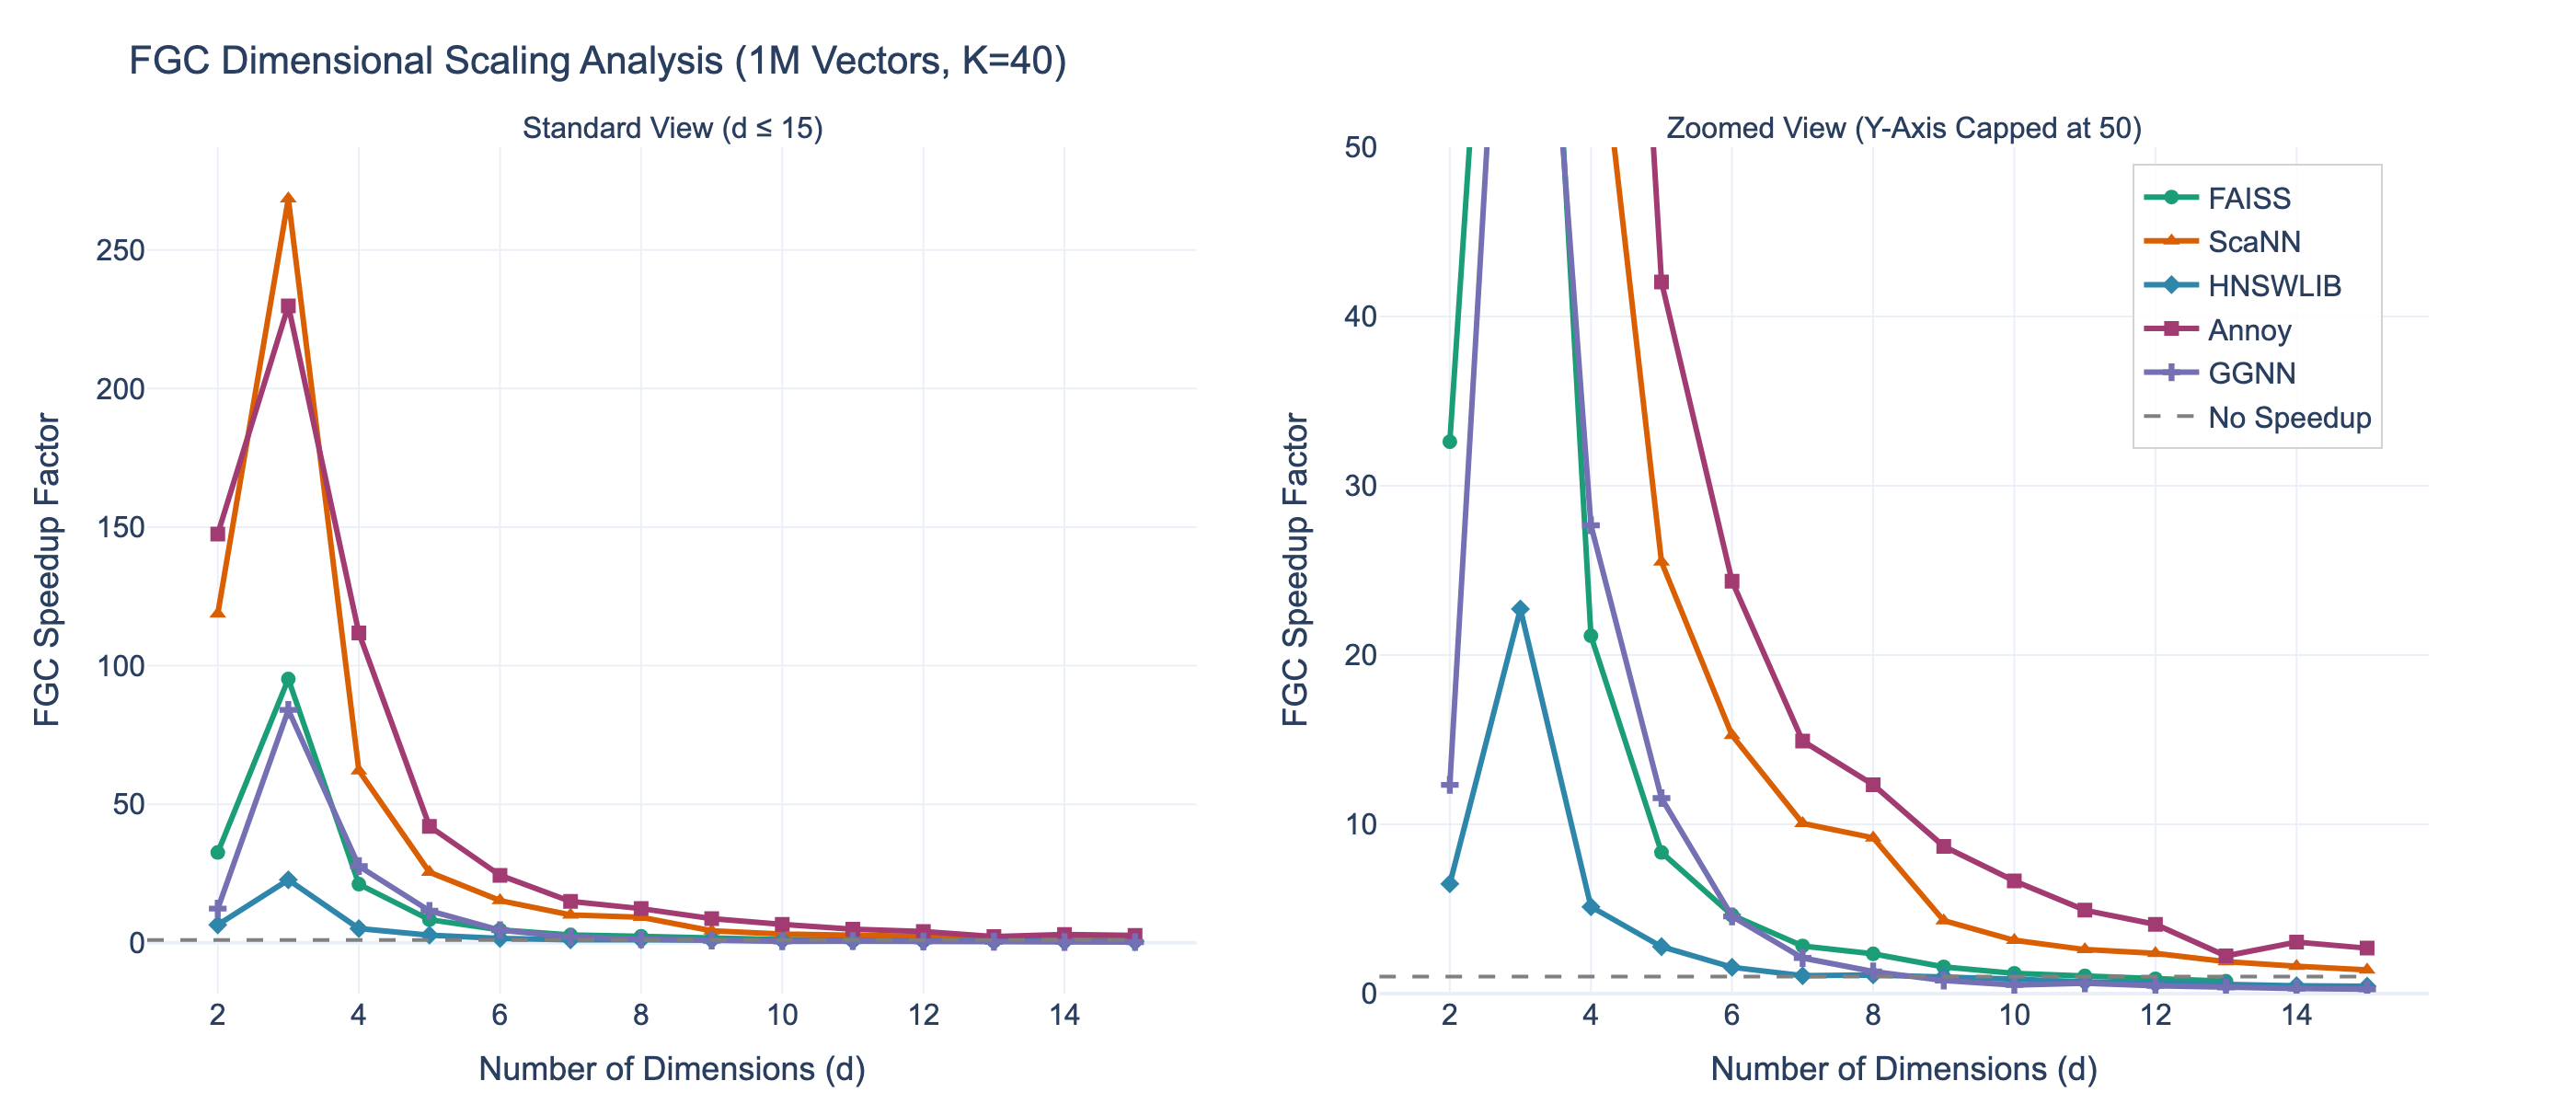
\includegraphics[width=0.85\textwidth]{synthetic_fgc_dimensional_scaling_1M_k40_all_algorithms.png}
  \caption{Controlled synthetic dimensional scaling at $N=1$M and $k=40$ on uniformly distributed vectors. FastGraph speedup over exact FAISS peaks at $d=3$ and decreases as dimensionality grows.}
  \label{fig:synthetic_dim_speedup}
\end{figure}

\begin{figure}[H]
\centering
  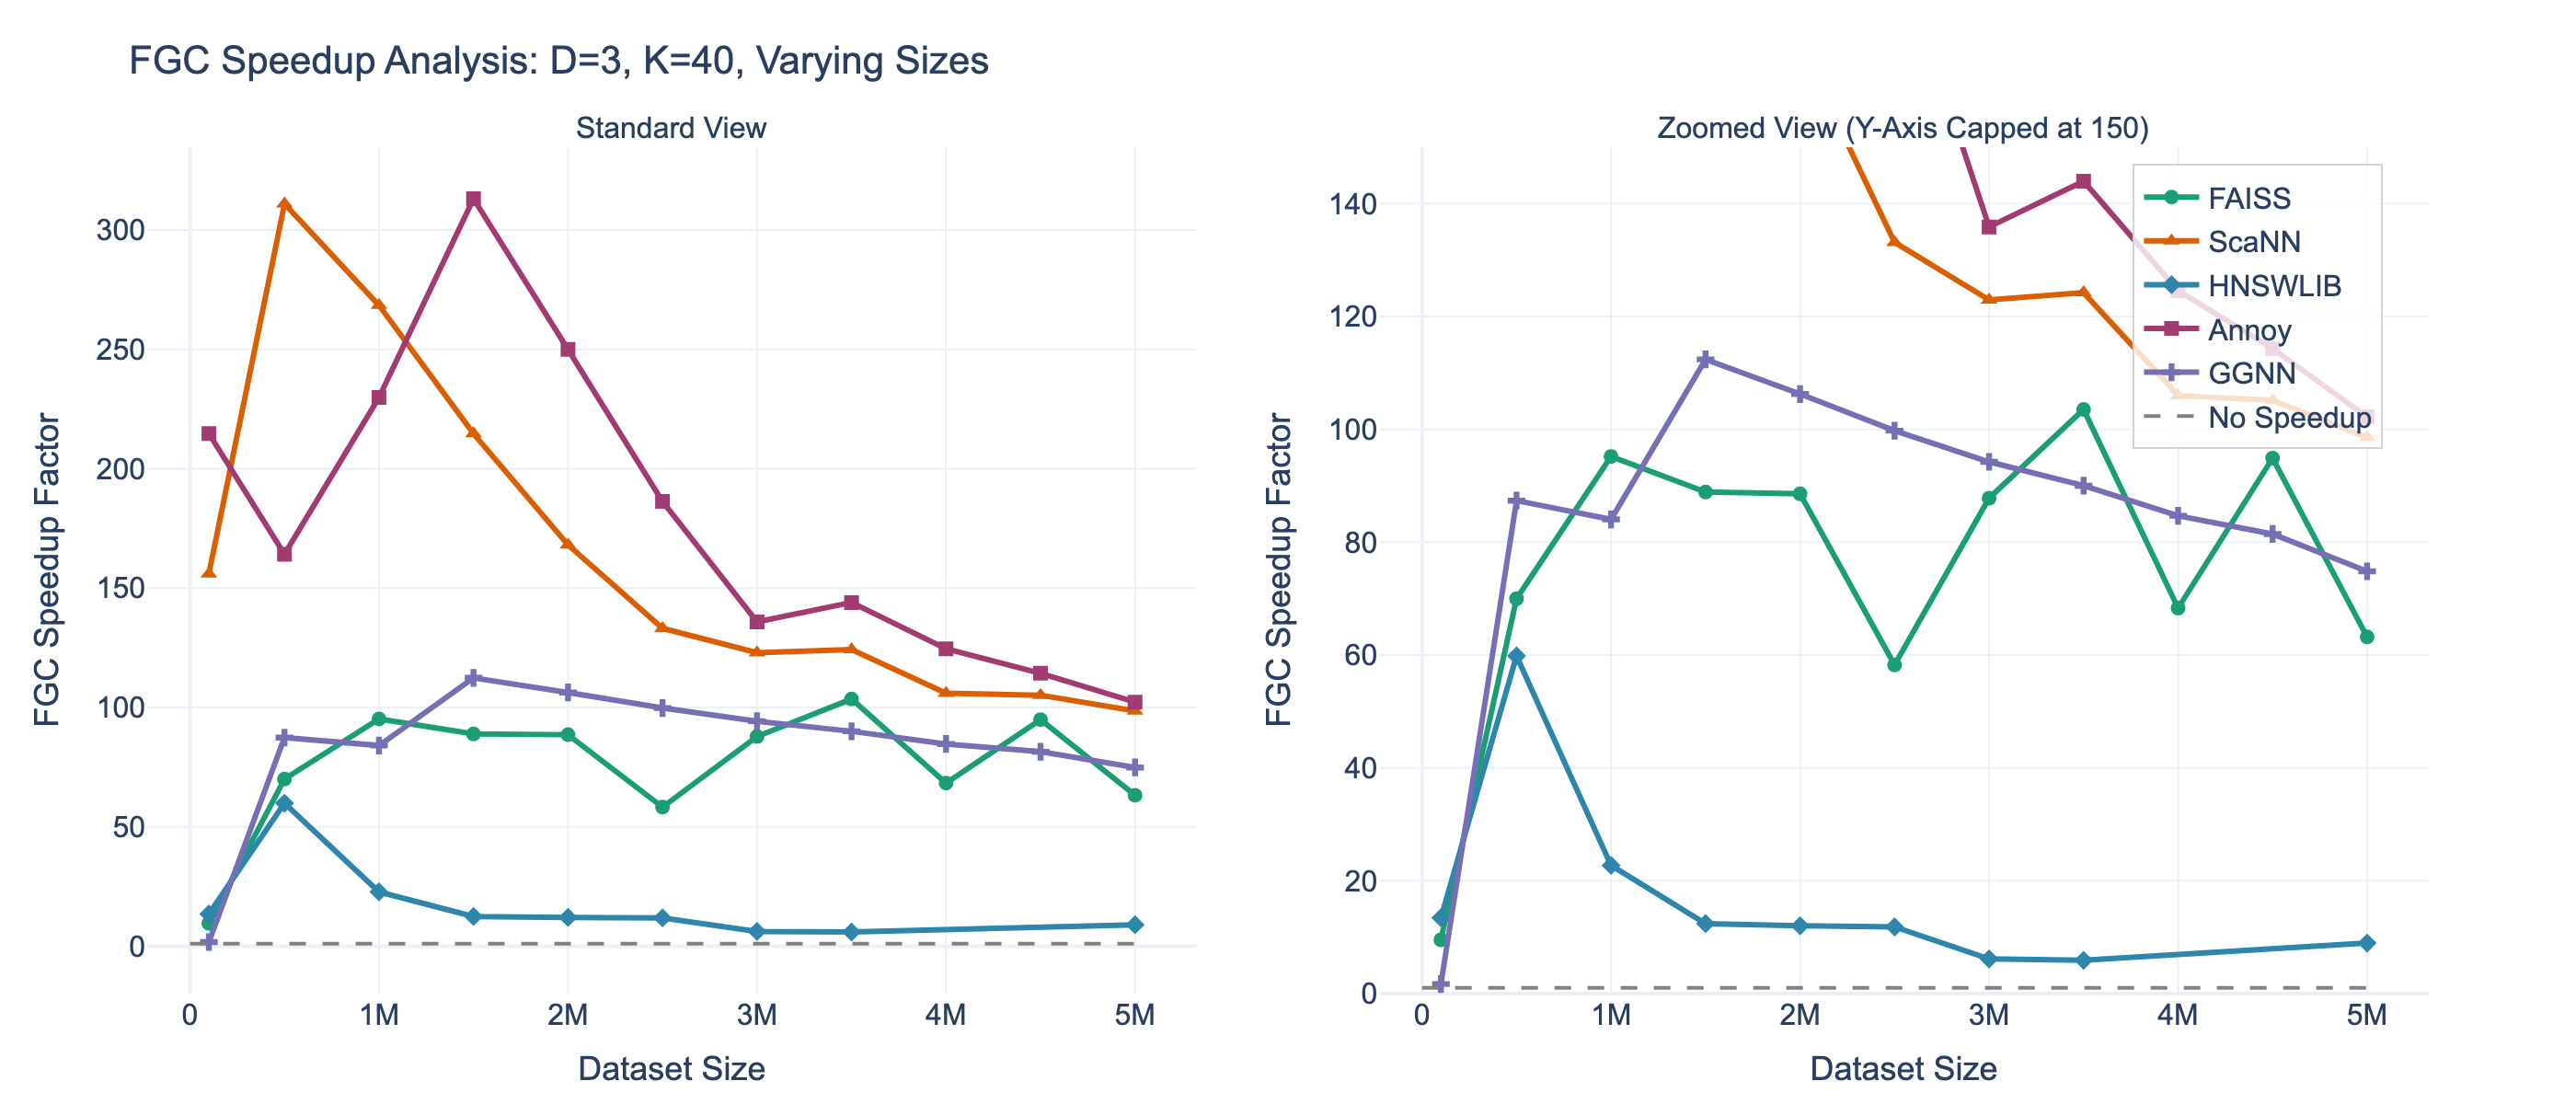
\includegraphics[width=0.85\textwidth]{synthetic_fgc_speedup_d3_all_algorithms.png}
  \caption{Controlled synthetic dataset-size scaling at $d=3$. FastGraph benefits most when dimensionality is low and the bin partition remains selective.}
  \label{fig:synthetic_speedup_d3}
\end{figure}

\begin{figure}[H]
\centering
  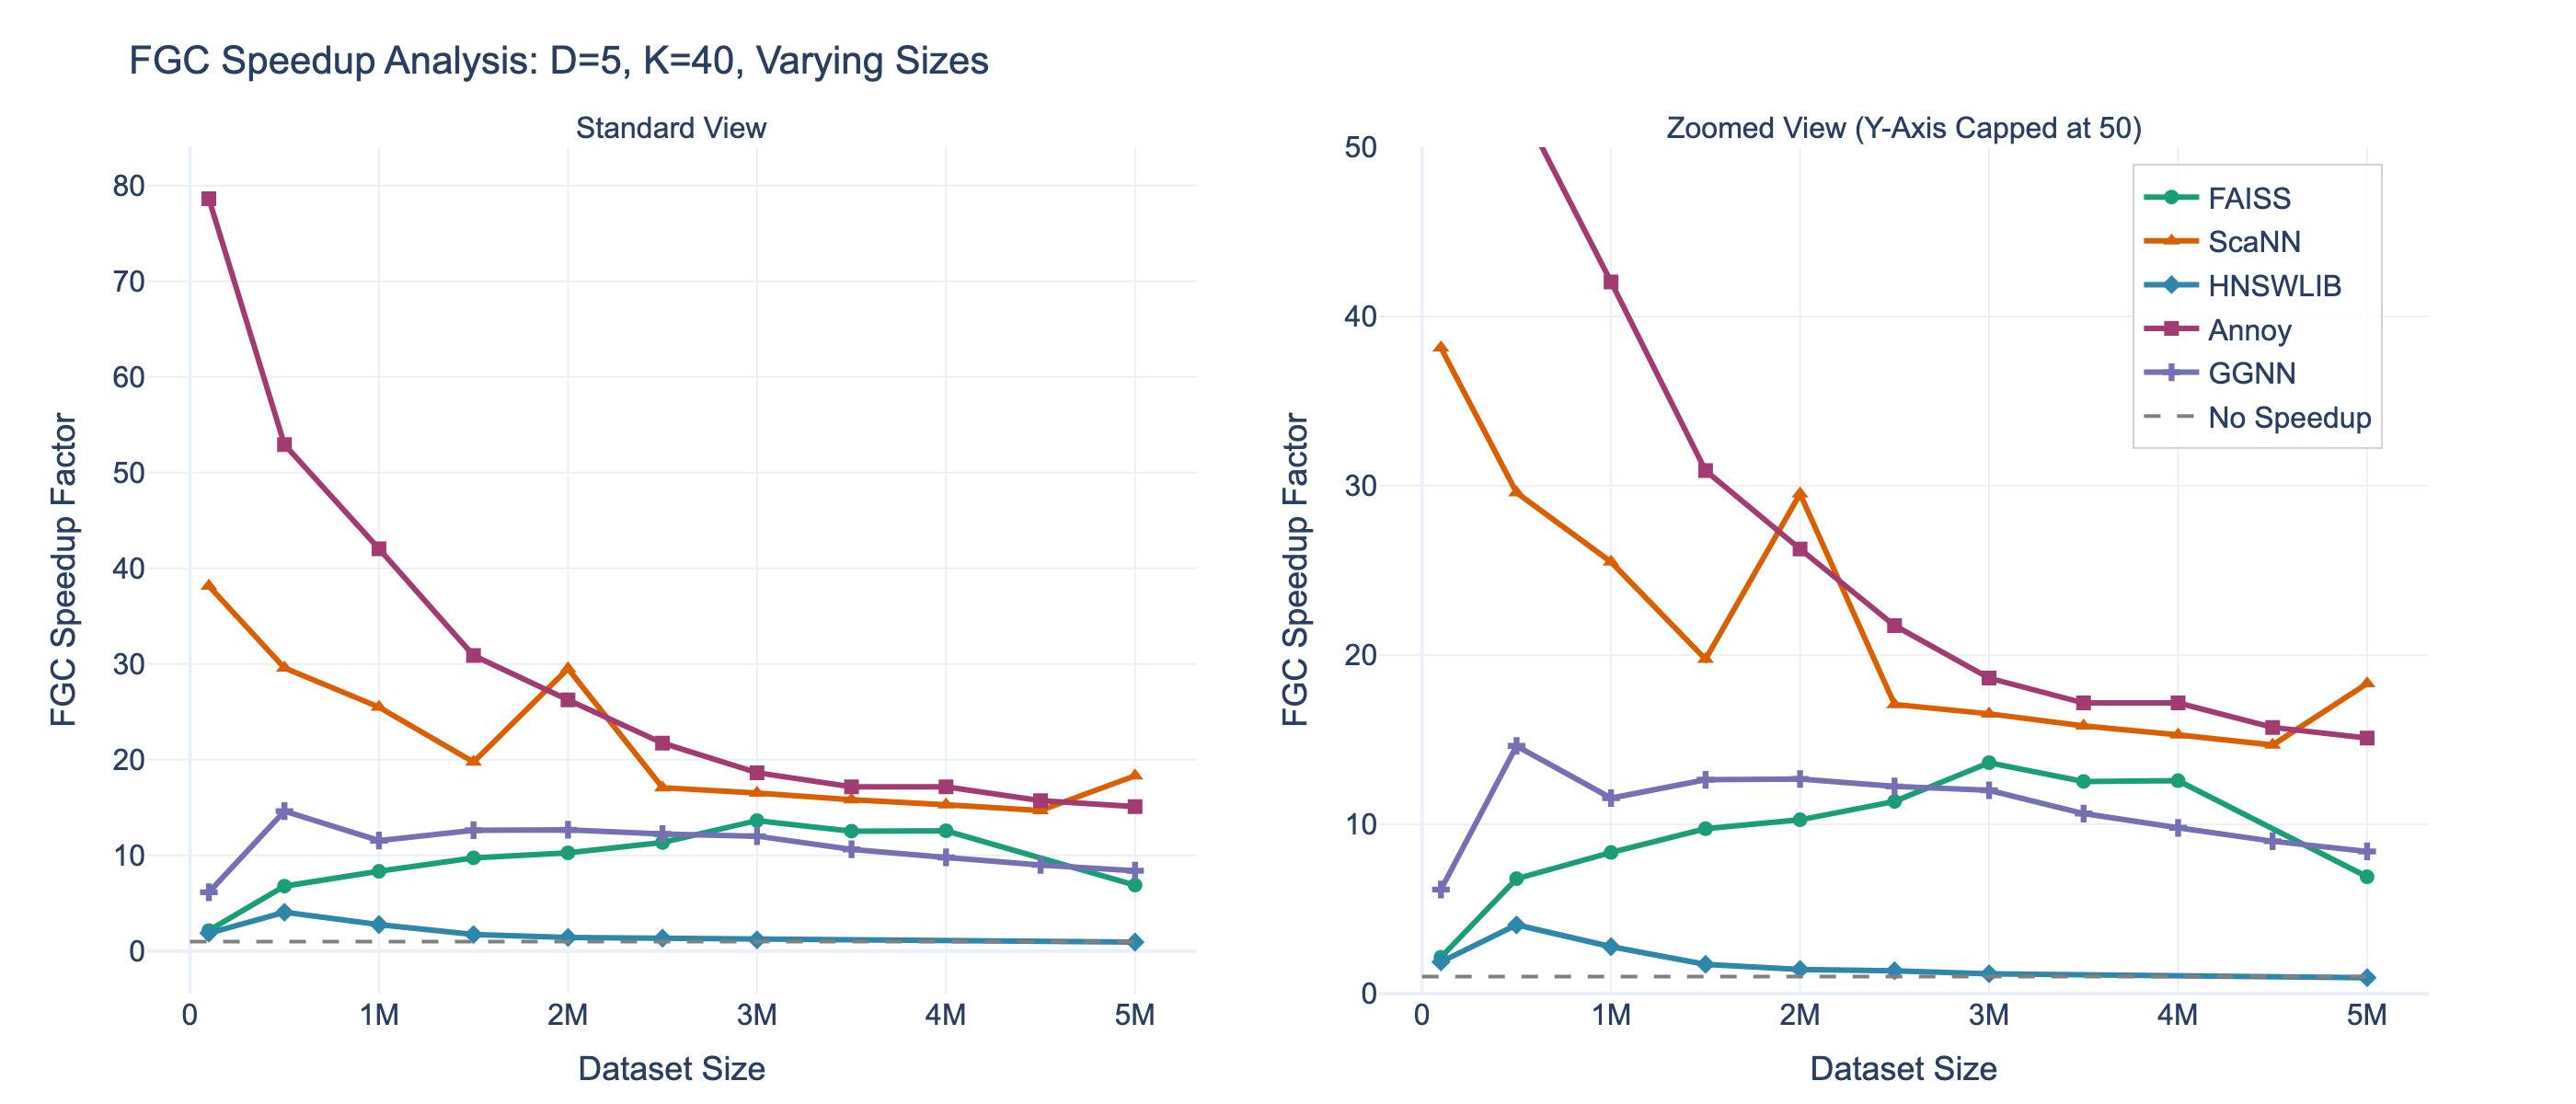
\includegraphics[width=0.85\textwidth]{synthetic_fgc_speedup_d5_all_algorithms.png}
  \caption{Controlled synthetic dataset-size scaling at $d=5$. The advantage is smaller than at $d=3$ but remains visible in the low-dimensional setting.}
  \label{fig:synthetic_speedup_d5}
\end{figure}

\subsection{Detector-Derived GPU Benchmarks}

We additionally benchmark on detector-derived point clouds drawn from CMS High Granularity Calorimeter (HGCAL) simulation data. The dataset consists of recHit feature vectors from 1.16 billion calorimeter hits across all events, with up to 10 spatial and energy features per hit. These workloads are less uniform than the synthetic data and include many spatially coincident hits from the same detector cell across events. This setting is closer to the target scientific application and therefore provides the most conservative estimate of end-to-end usefulness.

\begin{figure}[H]
\centering
  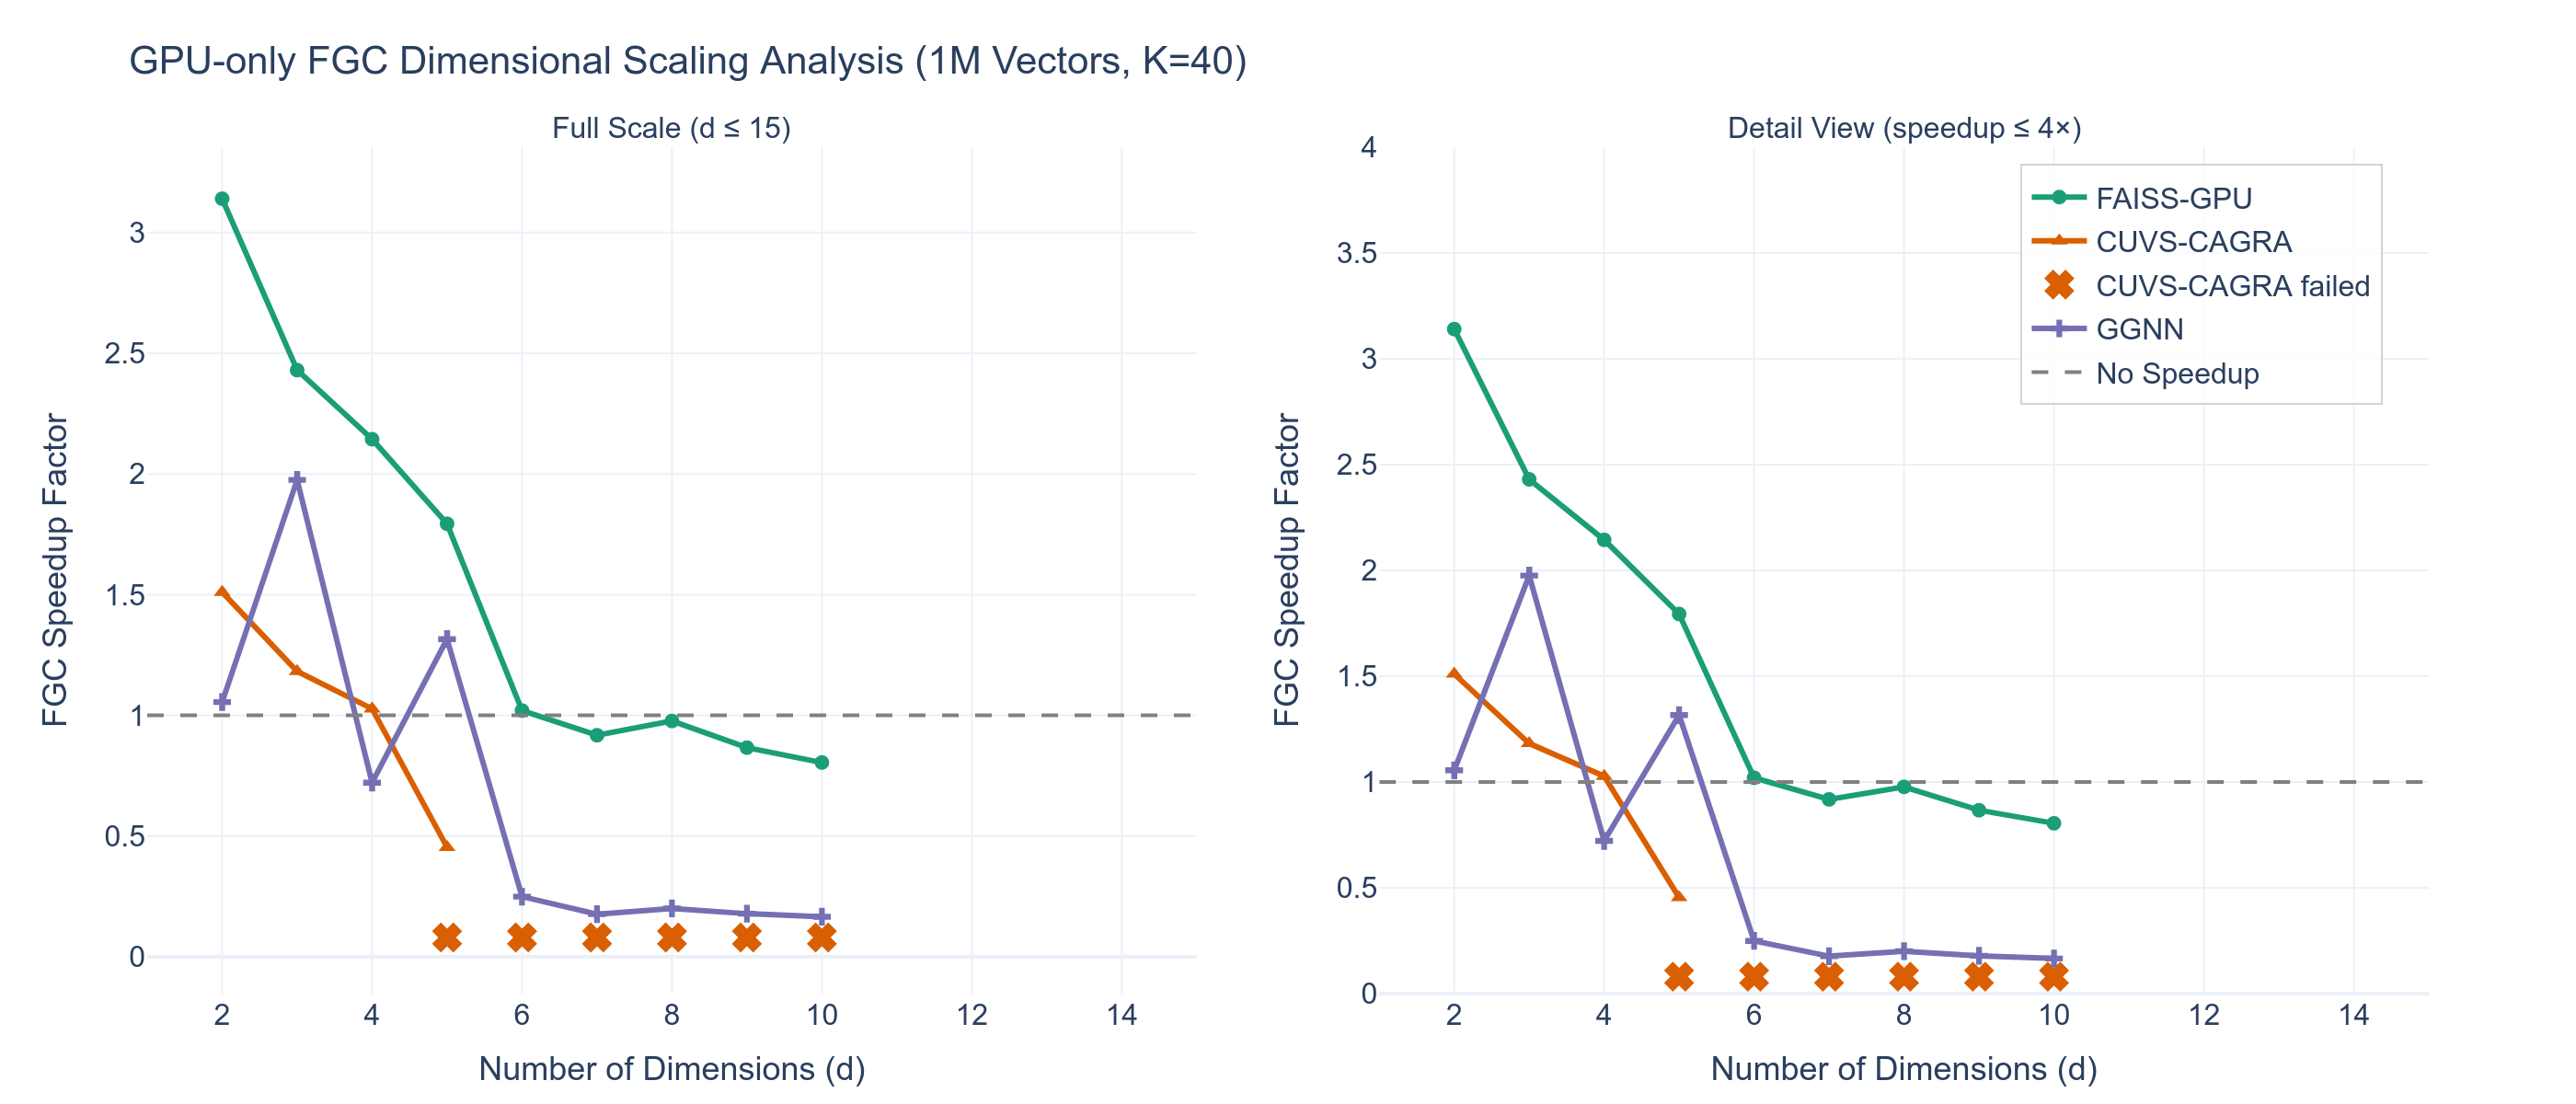
\includegraphics[width=0.85\textwidth]{gpu_fgc_dimensional_scaling_1M_k40_all_algorithms.png}
  \caption{Detector-derived GPU dimensional scaling at $N=1$M and $k=40$. FastGraph is fastest in the lowest-dimensional exact-search regime, while FAISS becomes preferable as dimensionality increases.}
  \label{fig:gpu_dim_speedup}
\end{figure}

At $N=1$M and $k=40$, FastGraph is approximately $3.1\times$ faster than exact FAISS \texttt{IndexFlatL2} at $d=2$, $2.1\times$ faster at $d=3$--$4$, and $1.8\times$ faster at $d=5$. At $d=6$ and above, FAISS and FastGraph reach near-parity or FAISS becomes faster, so FastGraph's advantage vanishes in the higher-dimensional regime. This trend is expected: FastGraph's candidate pruning depends on low-dimensional spatial locality, whereas FAISS's brute-force GPU kernel is less sensitive to data non-uniformity and becomes harder to beat as more dimensions are included.

GGNN, an approximate method, shows a dimension-dependent profile distinct from both exact methods: at $d=3$ its graph traversal is slower than FastGraph ($14.8$ vs $7.4$ s at $N=1$M, $k=40$), while at $d \geq 6$ it is substantially faster by operating with reduced recall. This confirms that for the exact-search regime FastGraph targets, GGNN is not a directly comparable baseline; the recall evaluation (Section~\ref{sec:recall}) quantifies this distinction explicitly.

\begin{figure}[H]
\centering
  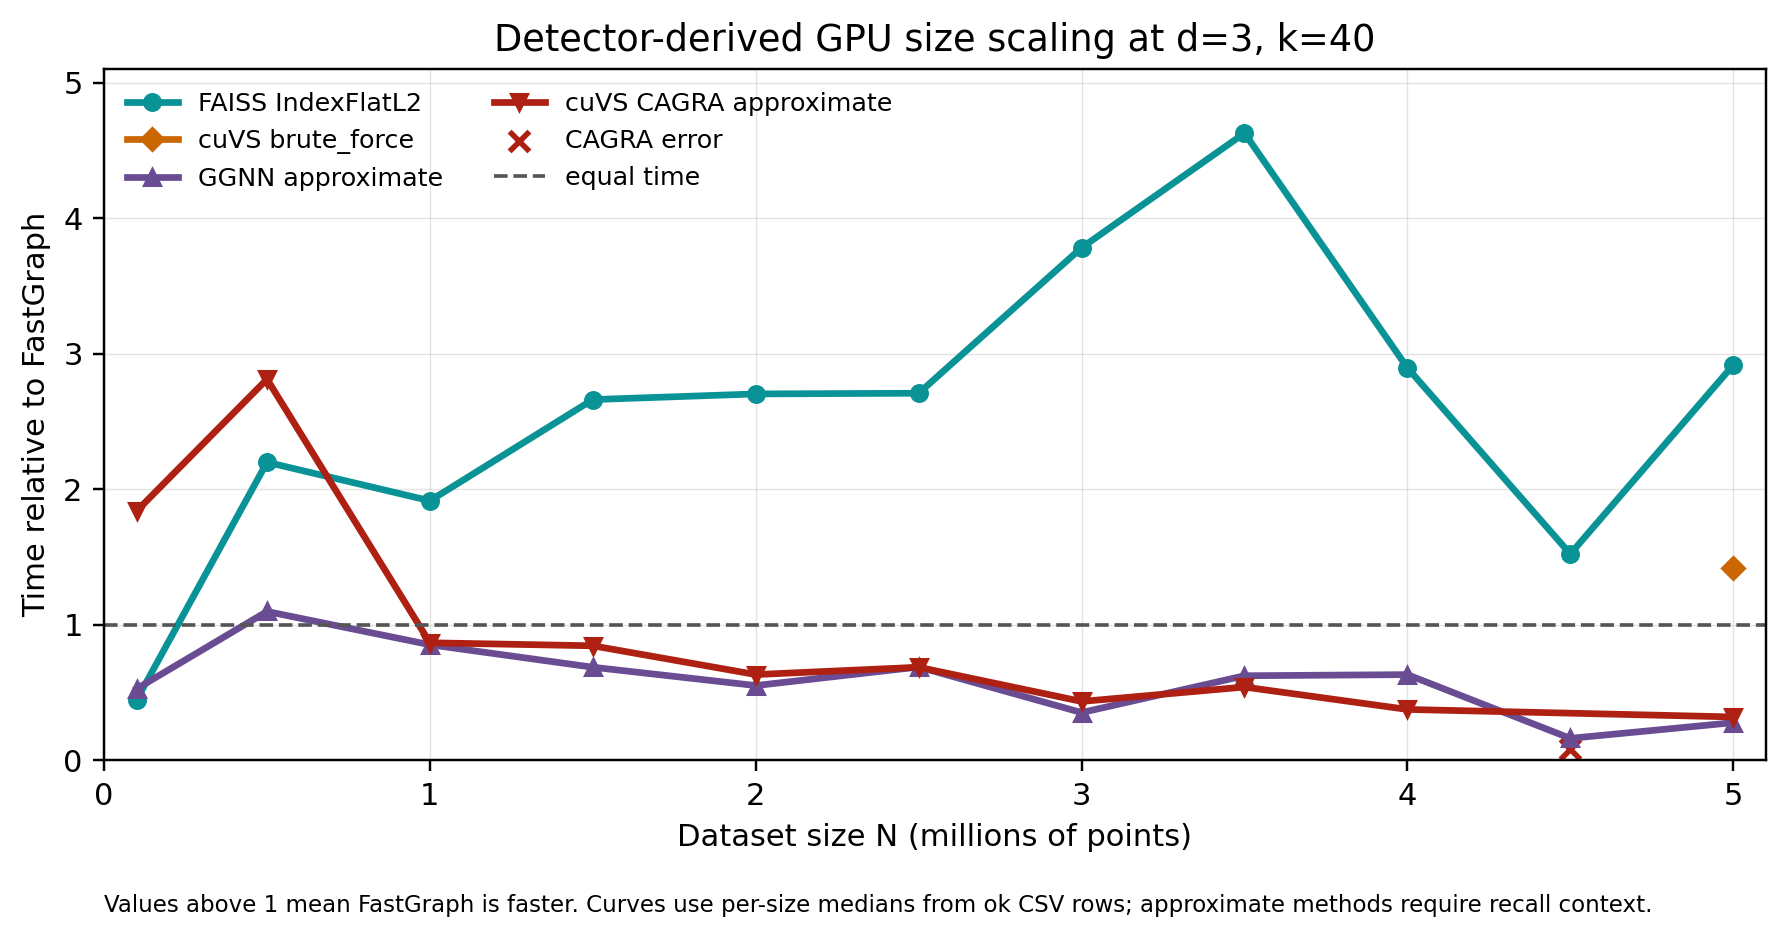
\includegraphics[width=0.85\textwidth]{gpu_fgc_speedup_d3_all_algorithms.png}
  \caption{Detector-derived GPU dataset-size scaling at $d=3$, $k=40$. FastGraph maintains a speed advantage over exact FAISS at $N \leq 3$M; the advantage diminishes at $N=5$M as both methods approach the same GPU throughput ceiling. GGNN is faster than exact methods at small $N$ but is an approximate method (recall $\approx 0.41$ at this configuration). cuVS CAGRA failures are shown as cross markers.}
  \label{fig:gpu_size_scaling_d3}
\end{figure}

\begin{figure}[H]
\centering
  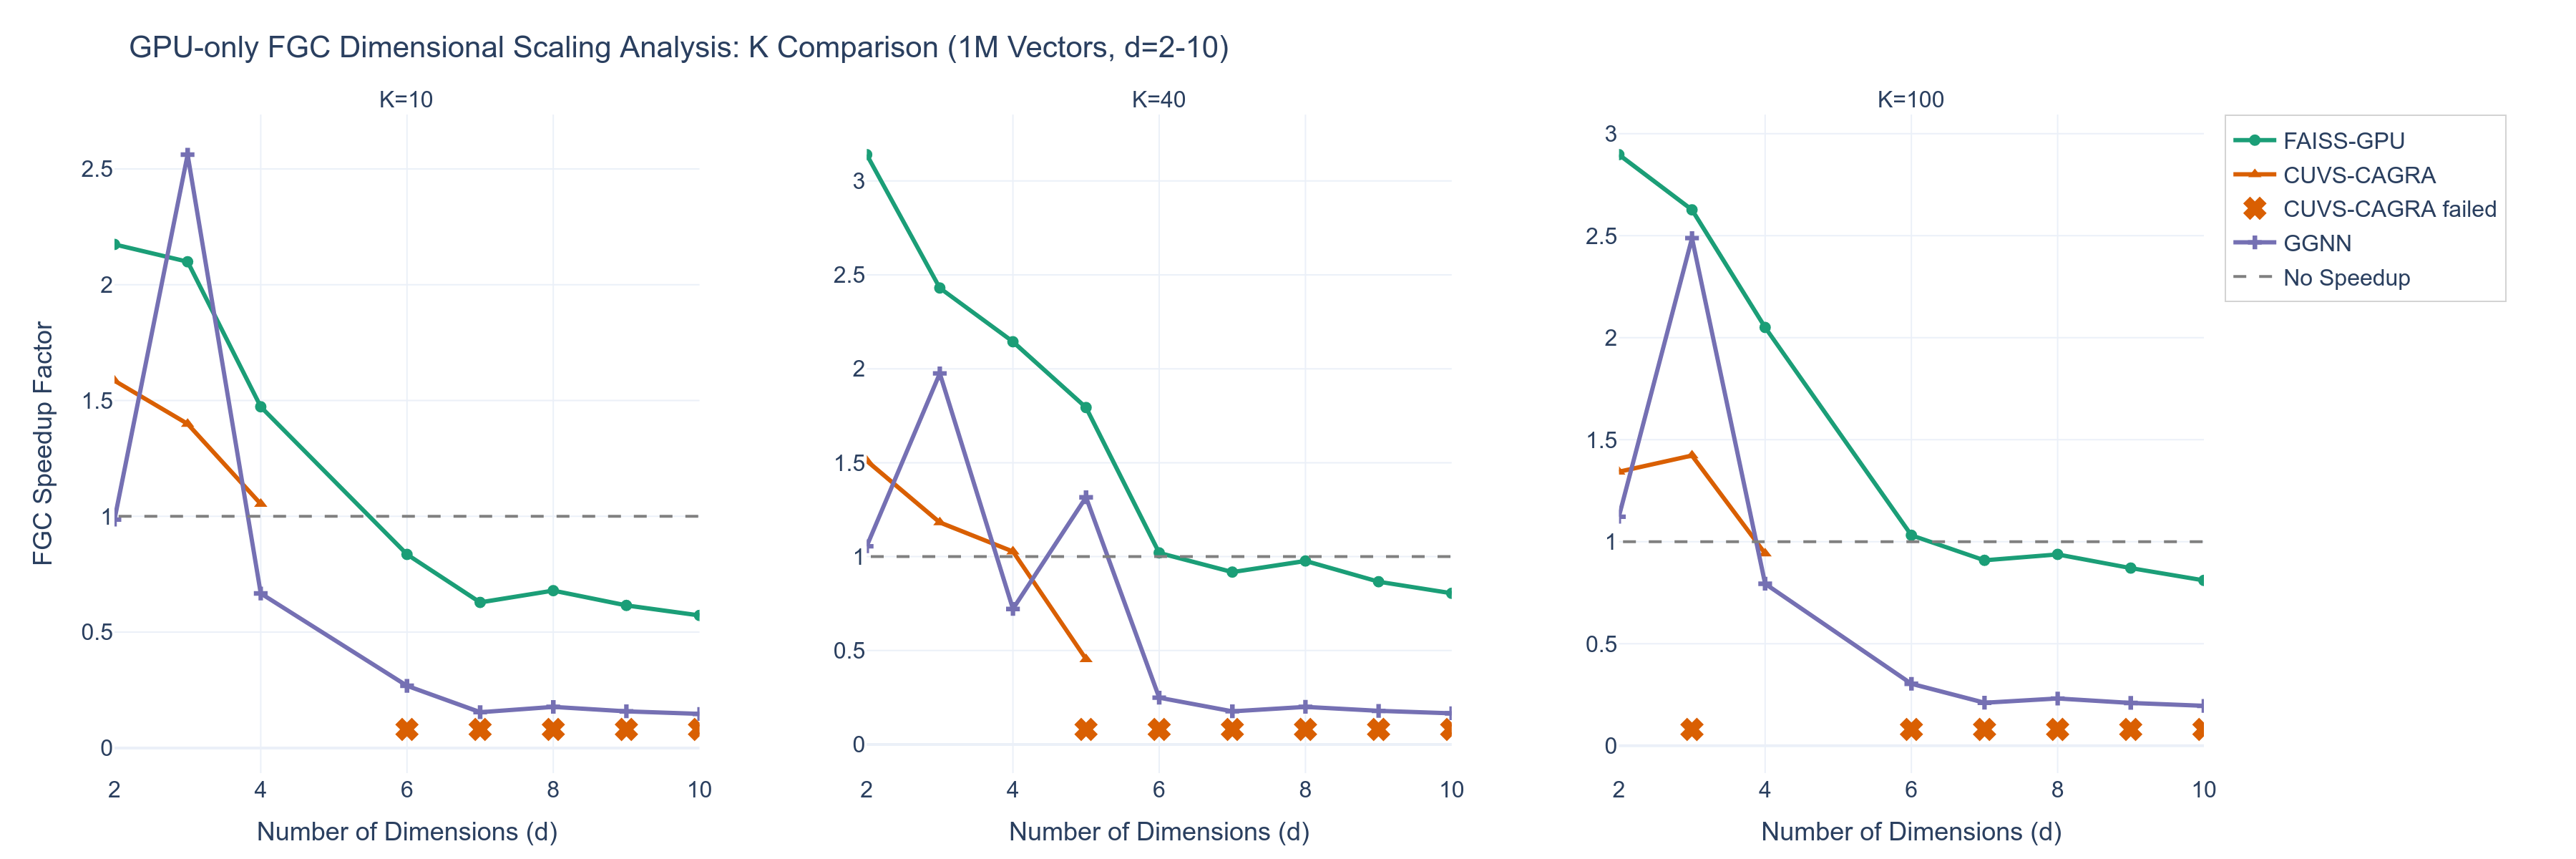
\includegraphics[width=0.95\textwidth]{gpu_fgc_k_comparison_1M_d2-10_all_algorithms.png}
  \caption{Detector-derived GPU speedup at $N=1$M for $k\in\{10,40,100\}$. Cross markers denote cuVS CAGRA configurations that returned benchmark errors rather than valid timings. The $d=5$, $k=10$ and $d=5$, $k=100$ rows are queued for rerun pending Slurm availability and are omitted from this figure.\protect\footnotemark}
  \label{fig:gpu_k_comparison}
\end{figure}
\footnotetext{The $d=5$, $k=40$ data is available and shows $1.8\times$ speedup over FAISS; the missing rows are expected to fall in the same range.}

Varying $k$ shows the same qualitative pattern: FastGraph is most useful in very low dimensions and at moderate neighborhood sizes. cuVS CAGRA fails on several detector-derived configurations because the intermediate CAGRA graph construction receives too many invalid or duplicated neighbor nodes, a behavior consistent with the high duplicate-coordinate rate in the data. We represent these failures explicitly in Fig.~\ref{fig:gpu_k_comparison} rather than silently dropping the series.

\subsection{Memory Footprint}

\begin{figure}[H]
\centering
  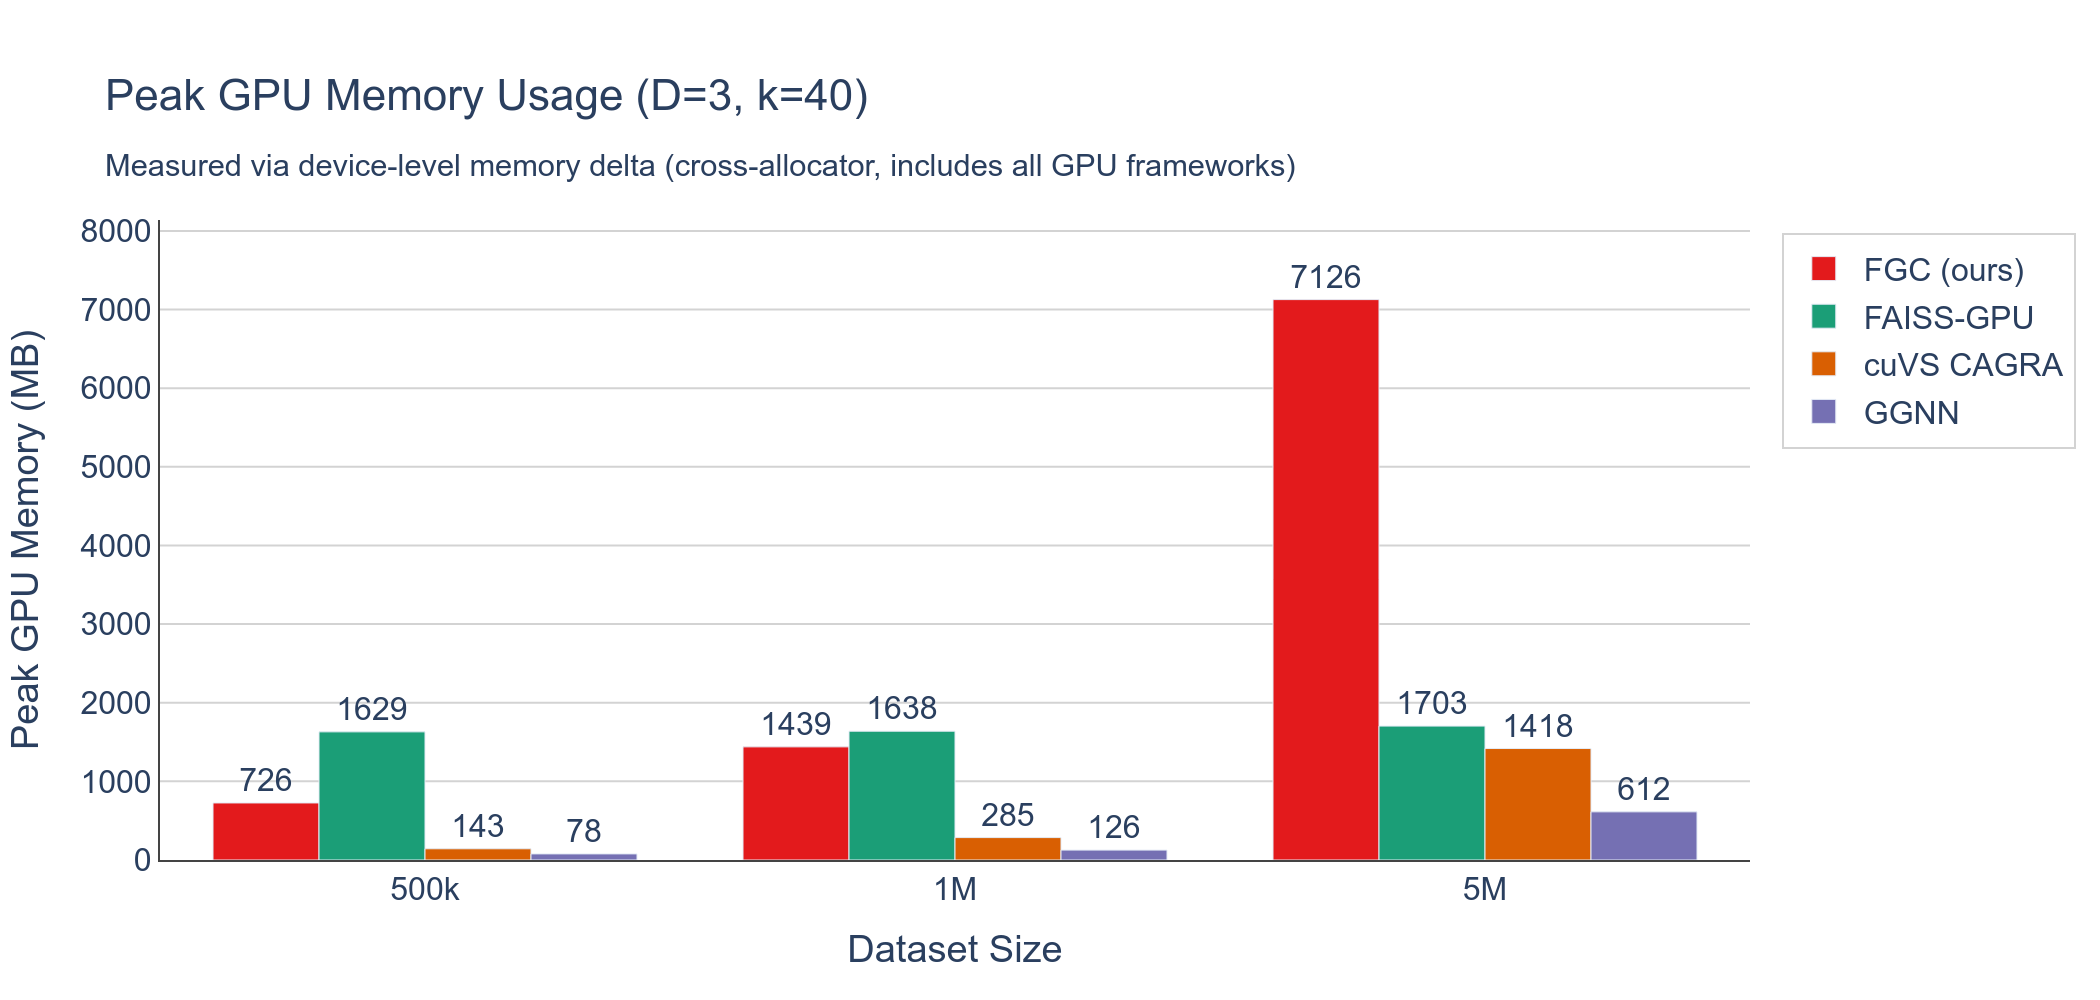
\includegraphics[width=0.85\textwidth]{memory_footprint.png}
  \caption{GPU memory footprint across dataset sizes. FastGraph's binning structures increase memory use at large $N$, so the method should be presented as a speed-memory tradeoff rather than as a zero-overhead replacement.}
  \label{fig:memory_footprint}
\end{figure}

FastGraph allocates bin assignments, bin boundaries, and intermediate structures whose size scales with both the number of points and the binning configuration. At large $N$, these structures add measurable GPU memory overhead above the base data allocation, as shown in Fig.~\ref{fig:memory_footprint}. FastGraph should therefore be understood as a speed-memory tradeoff: it exchanges additional GPU memory for exact low-dimensional search speed, and this tradeoff is most favorable in workloads where graph construction dominates runtime and latent spaces are intentionally low-dimensional.

\subsection{Recall Evaluation}
\label{sec:recall}

To verify that FastGraph produces exact $k$-nearest neighbors, we compute distance-based recall against a brute-force ground truth on HGCAL calorimeter data with up to $5\times10^5$ points. Standard set-match recall (fraction of predicted indices appearing in the ground-truth set) is inappropriate for this dataset because the HGCAL recHit data contains a large number of spatially coincident points---multiple detector hits at identical coordinates across events. When many points share the same distance to a query, any permutation among them is an equally valid $k$NN result, yet set-match recall penalizes algorithms that break ties differently from the reference.

We therefore adopt \emph{distance-based recall}: a predicted neighbor is counted as correct if its squared Euclidean distance to the query is at most the $k$-th ground-truth distance (plus a small relative tolerance for floating-point rounding). Both the ground truth and the evaluation use element-wise squared~$\ell_2$ computation, $\sum_i(a_i - b_i)^2$, rather than the BLAS expansion $\|a\|^2 + \|b\|^2 - 2\,a{\cdot}b$ used by \texttt{torch.cdist}. The BLAS form is faster but suffers from catastrophic cancellation when the true distance is small relative to the norms---precisely the regime of coincident HGCAL hits. Element-wise computation avoids this and matches the distance kernel used internally by FastGraph, ensuring the evaluation reflects the algorithm's true accuracy.

Under this metric, FastGraph achieves $\text{recall} = 1.0$ across all tested configurations ($d \in \{2{-}10\}$, $k \in \{10, 40, 100\}$, $N$ up to $5\times10^5$), confirming that it is an exact $k$NN algorithm. By contrast, cuVS~CAGRA and GGNN---both approximate methods---achieve mean recall of $0.73$ and $0.67$ respectively averaged across all tested configurations at their highest-quality parameter settings (\texttt{itopk\_size}$=512$ and $\tau_{\text{query}}=0.8$); recall varies by configuration, reaching $0.82$ for cuVS and $0.41$ for GGNN at the $d=3$, $N=5\times10^5$, $k=40$ point shown in Fig.~\ref{fig:recall_exactness}. Neither approximate method can reach $99\%$ recall at $N \geq 5\times10^5$. When these methods are tuned to maximise accuracy, their query times exceed those of FastGraph, eliminating the speed advantage they hold at default (low-recall) settings.

FAISS (\texttt{IndexFlatL2}) is also a brute-force exact algorithm and is included in the recall comparison. Because FAISS uses the BLAS expansion internally, we evaluate its recall against a BLAS-consistent brute-force ground truth rather than the element-wise ground truth used for FastGraph. This consistent-kernel evaluation methodology---each algorithm evaluated against ground truth computed with its own distance kernel---ensures that each exact method achieves $\text{recall} = 1.0$ by construction, and that any recall deficit observed in the approximate methods reflects genuine search approximation rather than numerical kernel mismatch.

\begin{figure}[H]
\centering
  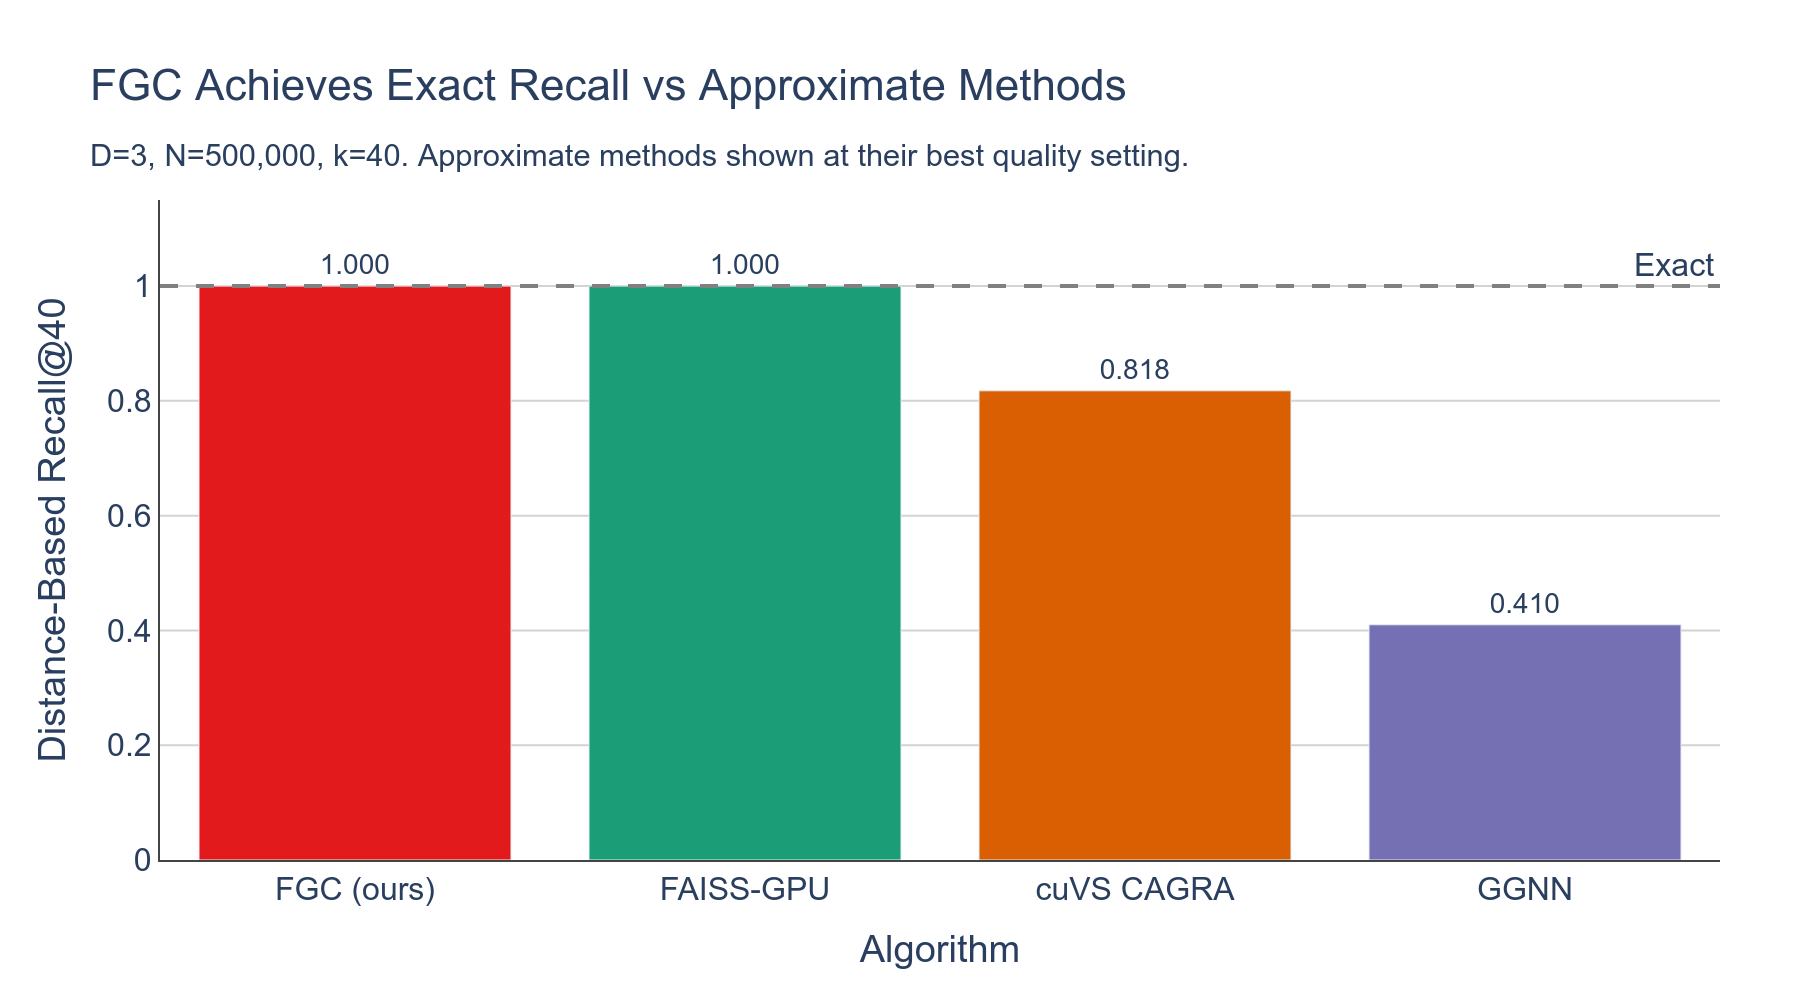
\includegraphics[width=0.85\textwidth]{recall_exactness_proof.png}
  \caption{Distance-based recall for FastGraph across detector-derived configurations. FastGraph returns exact nearest-neighbor distances under the tie-aware evaluation.}
  \label{fig:recall_exactness}
\end{figure}

\begin{figure}[H]
\centering
  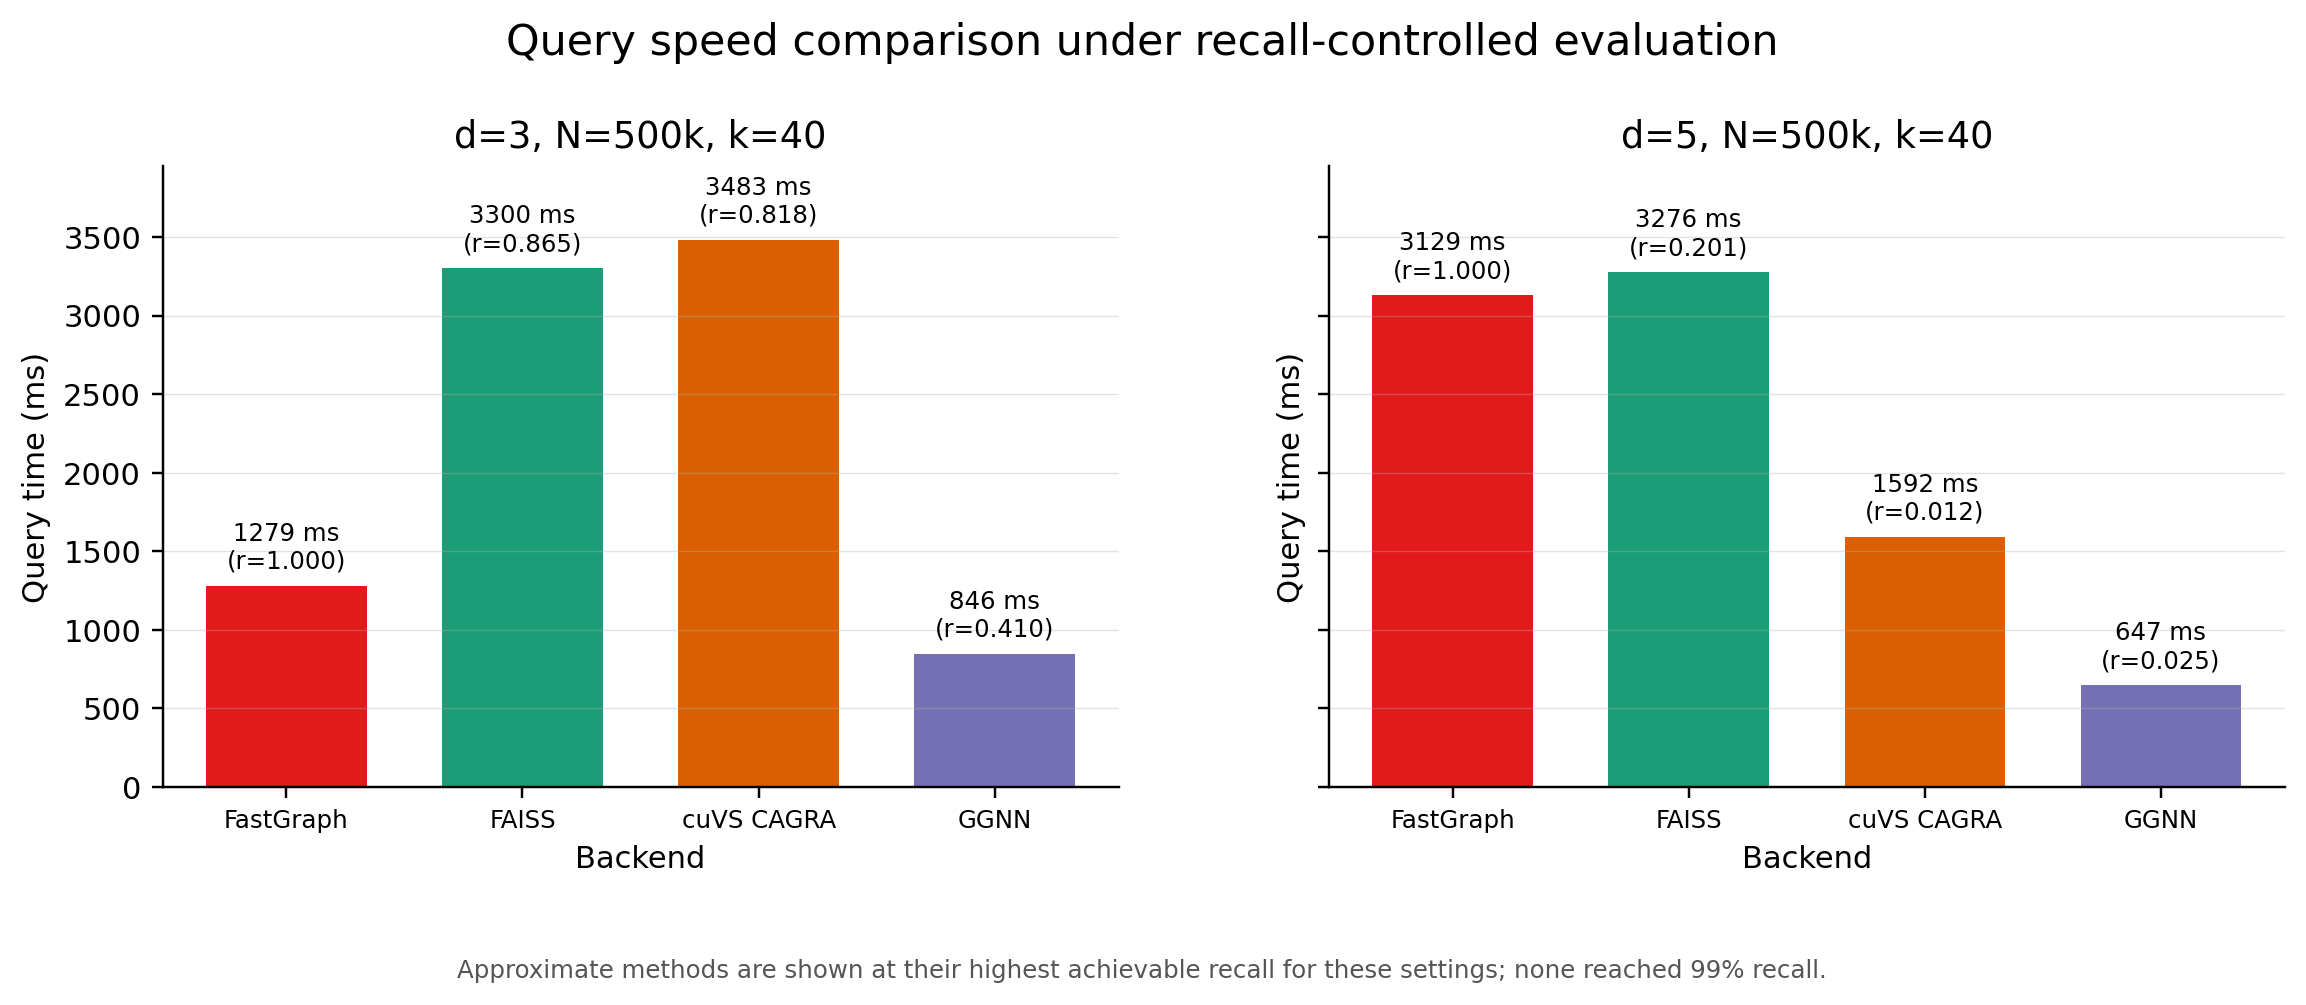
\includegraphics[width=0.85\textwidth]{recall_controlled_comparison.png}
  \caption{Recall comparison under controlled evaluation. Exact methods reach full recall under their corresponding distance kernels; approximate methods trade accuracy for query speed.}
  \label{fig:recall_comparison}
\end{figure}

\begin{figure}[H]
\centering
  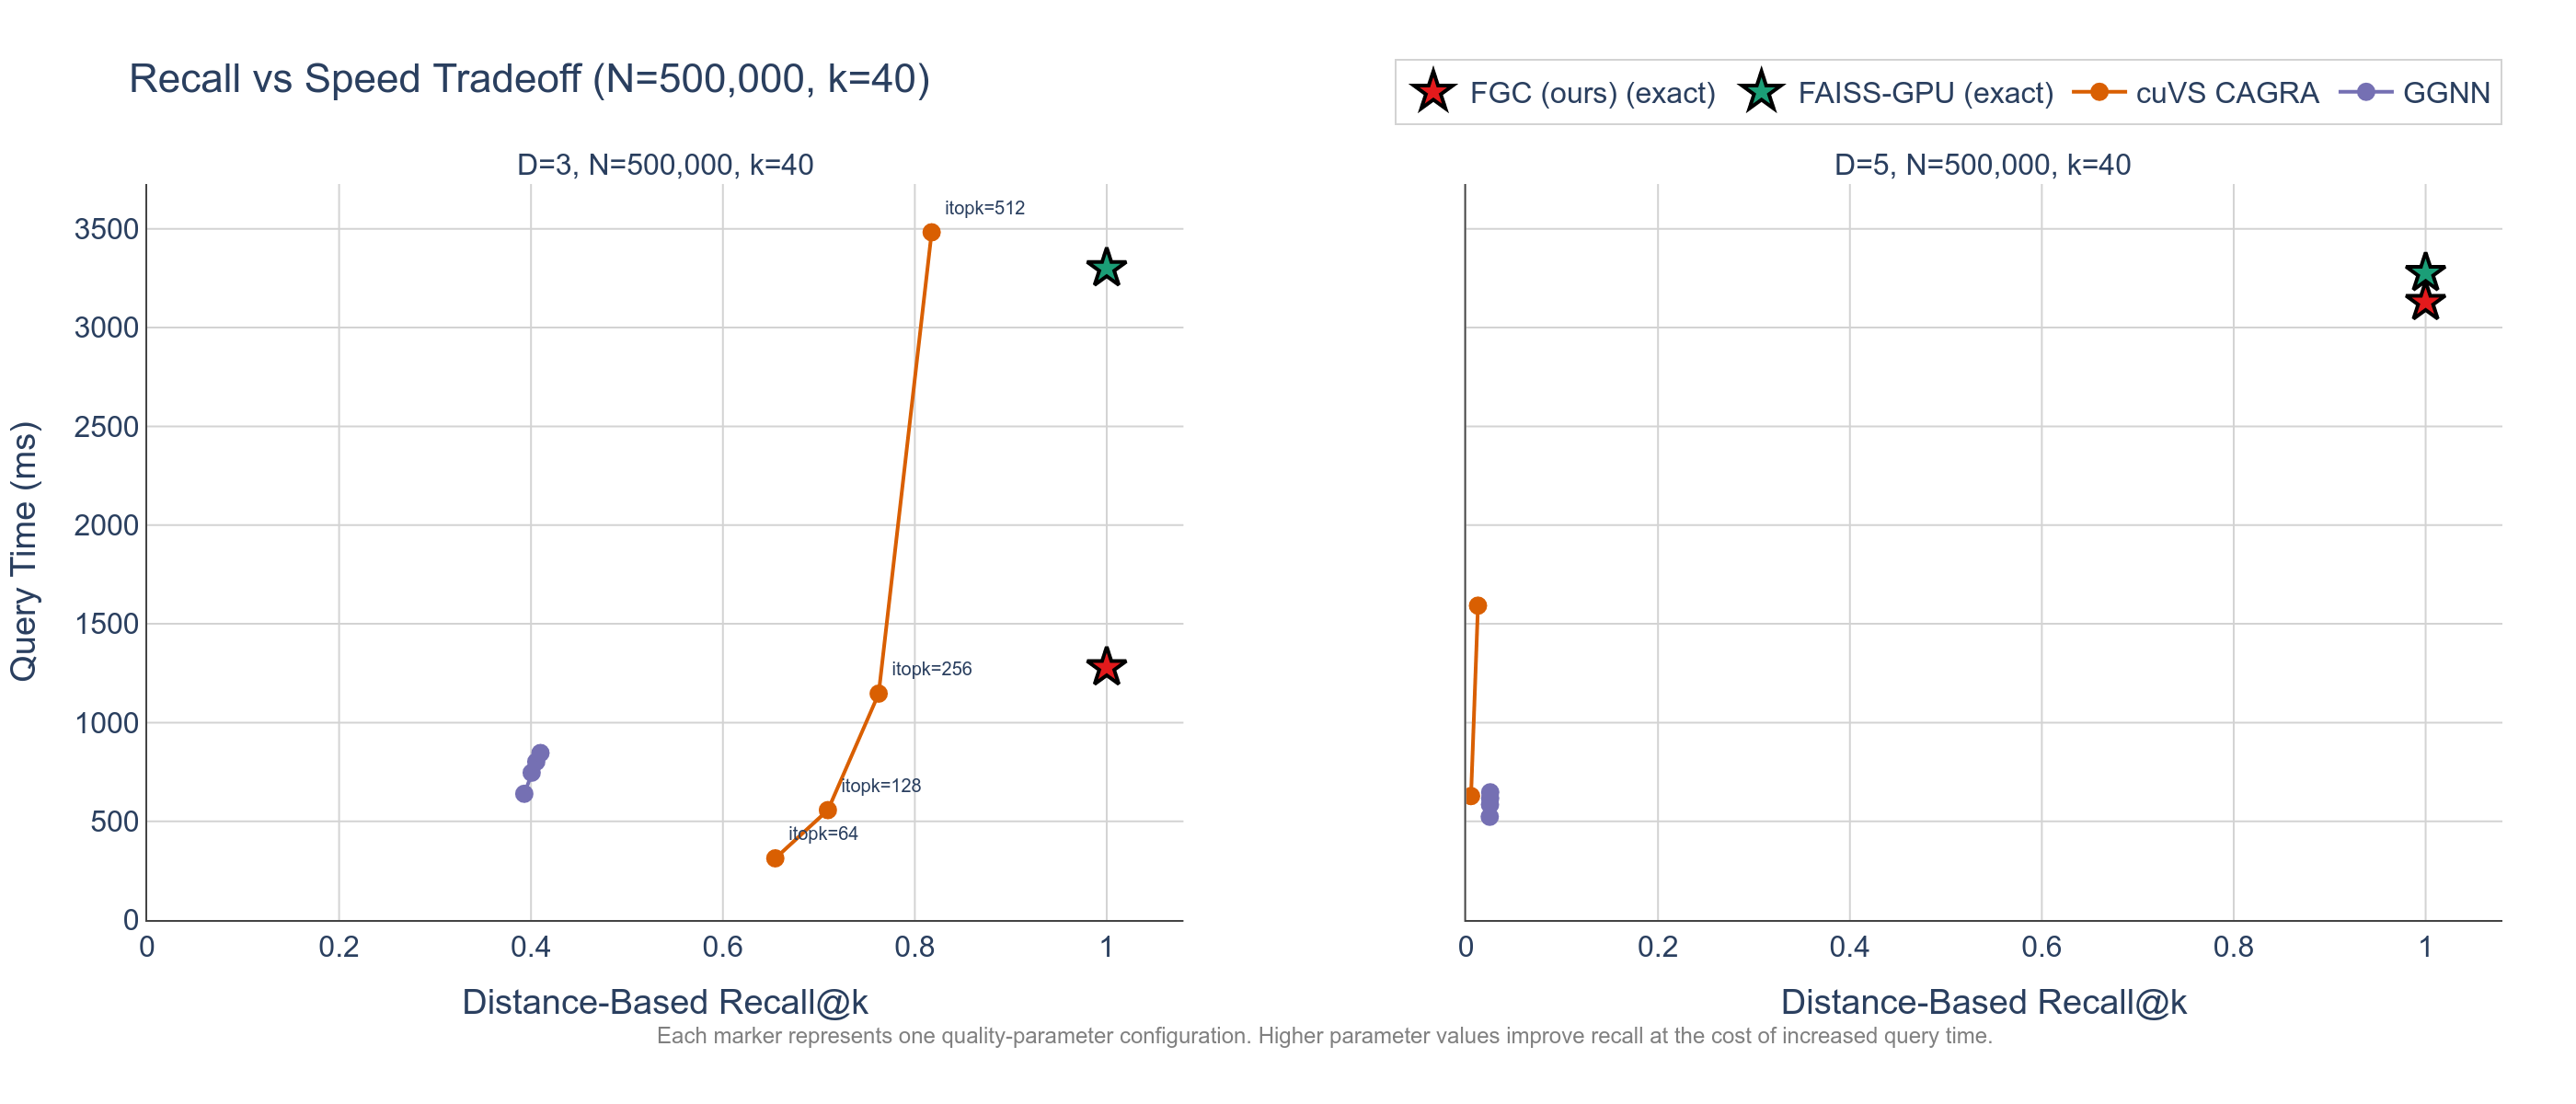
\includegraphics[width=0.85\textwidth]{recall_speed_pareto.png}
  \caption{Recall-speed tradeoff for exact and approximate methods. FastGraph occupies the exact, low-dimensional regime; approximate methods are only competitive when lower recall is acceptable.}
  \label{fig:recall_speed_pareto}
\end{figure}

\begin{figure}[H]
\centering
  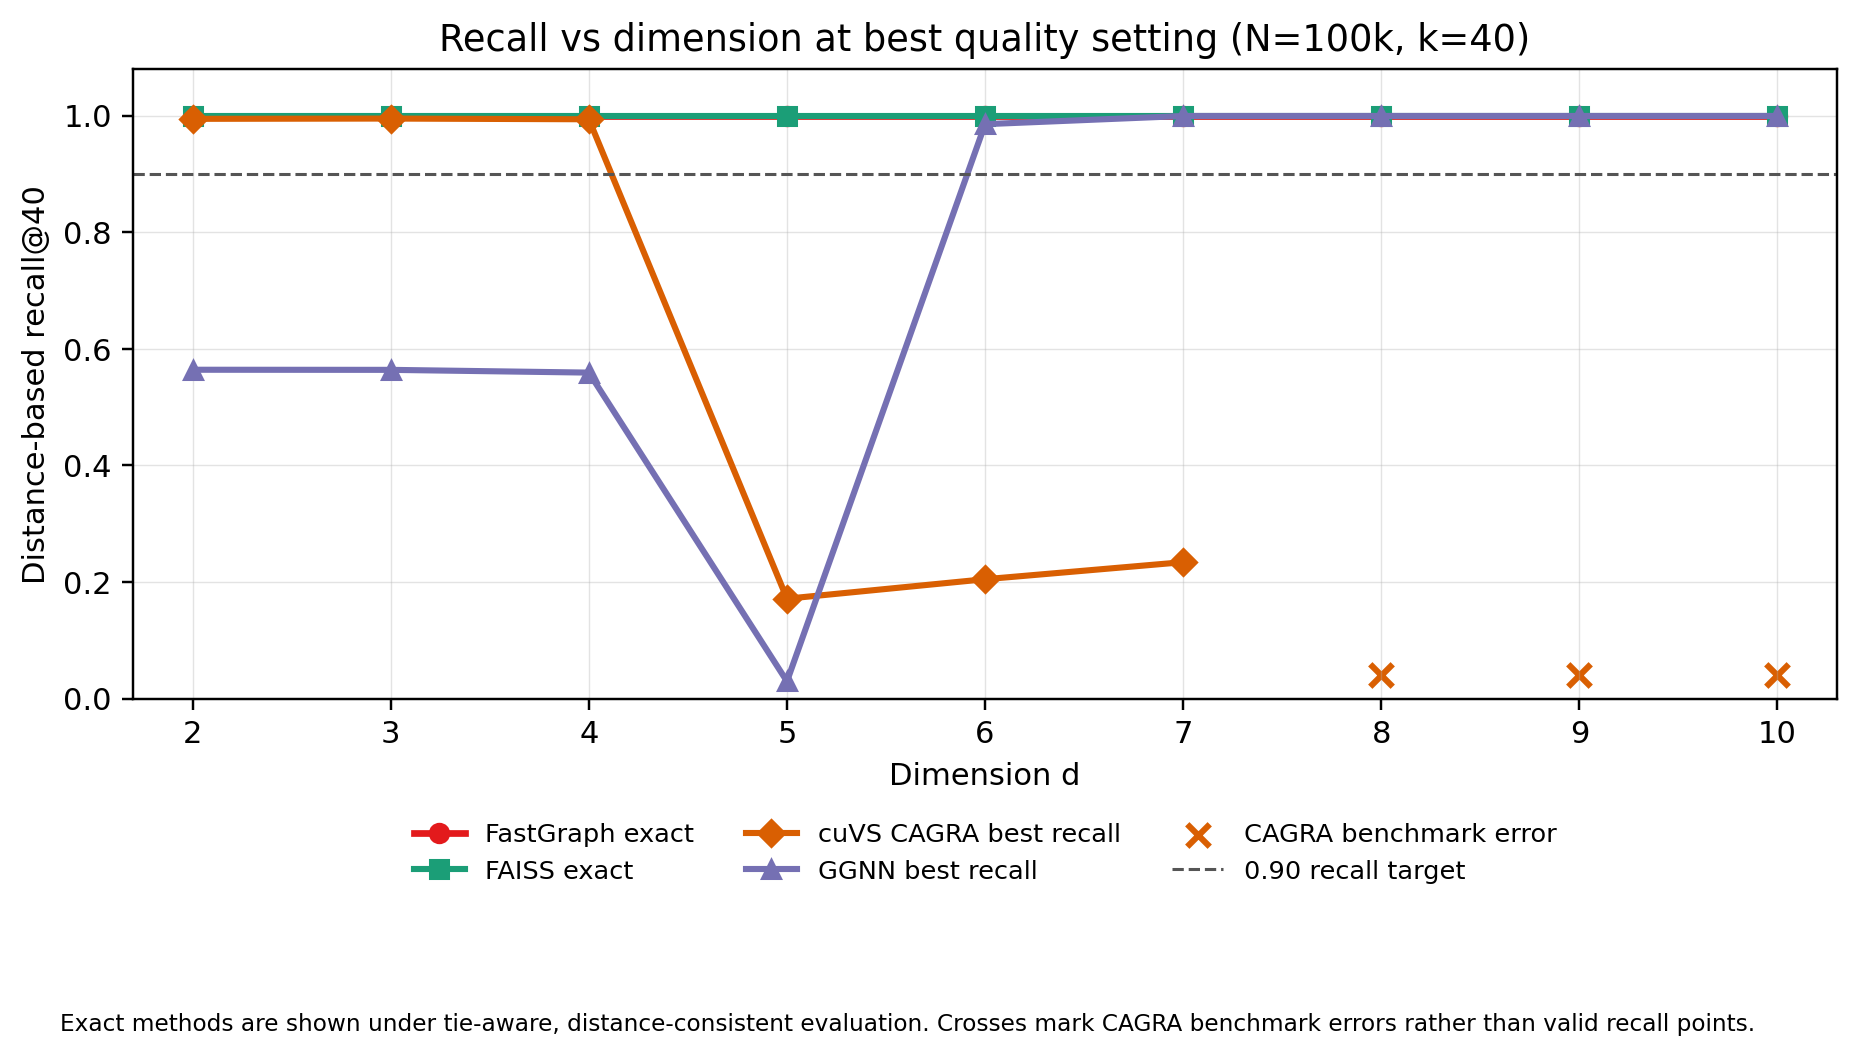
\includegraphics[width=0.85\textwidth]{recall_vs_dimension.png}
  \caption{Distance-based recall vs.\ dimension at best quality parameter settings ($N=10^5$, $k=40$). FastGraph maintains exact recall ($= 1.0$) across all tested dimensions. Both cuVS CAGRA and GGNN degrade significantly above $d=3$, with neither reaching 99\% recall at any dimension. Cross markers denote out-of-memory failures.}
  \label{fig:recall_vs_dimension}
\end{figure}

\subsection{Dynamic Graph Construction in GNNs}

Unlike traditional GNNs that operate on fixed graph structures, models such as \texttt{GravNet} dynamically construct edges by finding $k$-nearest neighbors in a learned latent space. This approach allows the network to adaptively form connections based on feature similarity rather than predetermined structural relationships. However, the computational cost of the $k$NN search has been a significant bottleneck, particularly for high-dimensional data or large batch sizes.

FastGraph integrates into GNN pipelines through \texttt{GravNetOp}, a complete GravNet layer that combines coordinate transformation, kNN graph construction, and message passing in a single autograd-compatible operation. Because \texttt{GravNetOp} uses the FastGraph kNN kernel internally, gradients propagate through the selected distances and point coordinates: these continuous quantities can be optimized jointly during training without any modification to the surrounding model. As discussed above, the hard neighbor indices are treated as fixed during each backward pass.

\section{Limitations}

FastGraph is designed for a specific operating regime and has several limitations that practitioners should consider before deployment.

\textbf{Dimensionality.} Spatial pruning via bin partitioning is effective only over the first $d_{\max} \leq 5$ dimensions. For inputs with $n_c > 5$, all dimensions participate in exact distance computation inside candidate bins, but the candidate pruning itself is blind to dimensions 6 and beyond. In high-dimensional latent spaces ($d \gtrsim 8$), the speedup over exact brute-force search diminishes and may vanish entirely, as confirmed by our detector-derived benchmarks at $d \geq 6$.

\textbf{Data distribution.} The bin partitioning assumes spatial locality: the speedup is largest when nearby points in feature space are likely to be mutual nearest neighbors. Highly non-uniform or clustered distributions reduce bin selectivity and can cause the search to degenerate toward brute force. The synthetic benchmarks (uniform data) therefore represent an upper bound on achievable speedup; real detector-derived data shows more conservative gains.

\textbf{Memory overhead.} FastGraph allocates auxiliary structures of size $O(N(n_c + K) + B)$ where $B = n_{\text{bins}}^{d_{\max}}$. At large $N$ and $d_{\max} = 5$, the bin boundary array alone can reach tens of millions of entries. FastGraph is not a zero-overhead drop-in for FAISS; the speed-memory tradeoff should be evaluated explicitly for each deployment.

\textbf{Single-GPU only.} The current implementation targets a single GPU. Multi-GPU or distributed kNN is not supported; for workloads that exceed single-GPU memory, FAISS's sharding utilities are more appropriate.

\textbf{Column ordering.} Bin partitioning always uses the first $d_{\max}$ feature columns. If the most discriminative dimensions are not among the first five, bin pruning will be less effective. A simple mitigation is to reorder columns by variance before calling FastGraph.

\textbf{Approximate-method comparison.} The benchmark comparison against cuVS CAGRA and GGNN is included to characterize the speed-accuracy tradeoff landscape, not to claim FastGraph is superior: both approximate methods are faster than FastGraph when lower recall is acceptable, and GGNN in particular is substantially faster at $d \geq 6$. FastGraph is the right choice only when exact neighbors are required.

\section{Data and Code Availability Statement}
The code implementing the proposed $k$NN algorithm, along with benchmarking scripts, configuration files, and synthetic data generation utilities, is publicly available at: \url{https://github.com/jkiesele/FastGraphCompute}
The exact version used in this paper corresponds to commit \texttt{f951f1e}. All synthetic datasets used in the experiments are generated on the fly using the provided scripts, which use fixed random seeds and configuration files included in the repository.
Instructions for reproducing all experiments are provided in the repository README.

The detector-derived benchmarks use CMS HGCAL simulation data (recHit feature vectors) accessed via an internal collaboration dataset. The feature layout consists of up to 10 spatial and energy features per calorimeter hit. Access to this dataset is available to CMS collaboration members; interested external parties should contact the corresponding author.

\section{Conclusion}
In this paper, we present FastGraph, a GPU-optimized $k$-nearest neighbor algorithm specifically designed for low-dimensional spaces (2-10 dimensions) prevalent in graph neural network applications. We introduce an adaptive bin-partitioning strategy with compile-time specialization and autograd support for the selected distances and coordinates. FastGraph is an exact graph-construction primitive that substantially accelerates low-dimensional workloads, achieving order-of-magnitude speedups on controlled synthetic data and more conservative $2$--$3\times$ gains on detector-derived million-point GPU workloads at $d=2$--4. The method is not uniformly faster across all dimensions and does not have negligible memory overhead at scale; instead, it trades additional GPU memory for exact low-dimensional speed. This makes FastGraph most compelling for scientific GNN workloads where latent spaces are intentionally low-dimensional and exact neighbor distances matter for training and evaluation.

\bibliographystyle{elsarticle-num}
\bibliography{references}

\appendix

\section{Object Condensation Helper — Implementation Details}
\label{app:oc}

In addition to $k$NN, the library provides a GPU-optimized CUDA kernel for the object condensation method~\cite{Kieseler2020ObjectCondensation}. Object condensation is widely used in particle physics to cluster sensor-hit point clouds into particle candidates. Its training loop requires two dense auxiliary index matrices to be recomputed at every forward pass:

\begin{enumerate}
  \item The \emph{association matrix} $M \in \mathbb{Z}^{n_{\text{unique}} \times n_{\max uq}}$, whose $k$-th row lists the vertex indices assigned to the $k$-th object candidate.
  \item The optional \emph{complement matrix} $M_{\lnot} \in \mathbb{Z}^{n_{\text{unique}} \times n_{\max rs}}$, listing vertices \emph{not} assigned to the candidate; required only when the repulsive term $m_{\lnot}$ is included in the loss.
\end{enumerate}

Both matrices must be recomputed every forward pass because the predicted associations and the ragged batch layout change from iteration to iteration. The CUDA kernel parallelizes over unique object candidates, assigning one thread per candidate. This eliminates atomic operations and thread synchronization, ensuring collision-free writes to the output matrices at the cost of $O(n_{\text{unique}})$ launched threads per forward pass.

\begin{algorithm}[H]
\DontPrintSemicolon
\KwIn{\texttt{asso\_idx}[$n_v$], \texttt{unique\_idx}[$n_u$], \texttt{unique\_rs\_asso}[$n_u$], \texttt{rs}[$n_s{+}1$], $n_v, n_u, n_{\max uq}, n_{\max rs}$, flag \texttt{calc\_m\_not}}
\KwOut{$M$[$n_u$][$n_{\max uq}$], $M_{\lnot}$[$n_u$][$n_{\max rs}$]}
$k \leftarrow \texttt{blockIdx.x} \cdot \texttt{blockDim.x} + \texttt{threadIdx.x}$\;
\If{$k \geq n_u$}{\Return}
$uq \leftarrow \texttt{unique\_idx}[k]$;\quad
$split \leftarrow \texttt{unique\_rs\_asso}[k]$;\quad
$start \leftarrow \texttt{rs}[split]$;\quad
$end \leftarrow \min(\texttt{rs}[split{+}1],\; n_v)$\;
\If{$end - start > n_{\max rs}$}{$end \leftarrow start + n_{\max rs}$}
$fill \leftarrow 0$\;
\For{$i \leftarrow start$ \KwTo $end-1$}{
  \If{$\texttt{asso\_idx}[i] = uq$}{
    $M[fill][k] \leftarrow i$;\quad $fill \leftarrow fill + 1$\;
    \If{$fill \geq n_{\max uq}$}{\Break}
  }
}
\While{$fill < n_{\max uq}$}{$M[fill][k] \leftarrow -1$;\quad $fill \leftarrow fill + 1$}
\If{\texttt{calc\_m\_not}}{
  $fill \leftarrow 0$\;
  \For{$i \leftarrow start$ \KwTo $end-1$}{
    \If{$\texttt{asso\_idx}[i] \neq uq$}{
      $M_{\lnot}[fill][k] \leftarrow i$;\quad $fill \leftarrow fill + 1$\;
      \If{$fill \geq n_{\max rs}$}{\Break}
    }
  }
  \While{$fill < n_{\max rs}$}{$M_{\lnot}[fill][k] \leftarrow -1$;\quad $fill \leftarrow fill + 1$}
}
\caption{CUDA Object Condensation Helper (\texttt{oc\_helper}): one thread per candidate.}
\label{alg:oc}
\end{algorithm}

\end{document}
